%% If you have any problems using this template, please contact the author: %%
%% Chris Carmona: carmona@stats.ox.ac.uk ; chriscarmona.me %%

\documentclass{beamer}

% fonts
\usepackage[scaled=0.92]{helvet}   % set Helvetica as the sans-serif font
\renewcommand{\rmdefault}{ptm}     % set Times as the default text font

% dmb: not mandatory, but i recommend you use mtpro for math fonts.
% there is a free version called mtprolite.

% \usepackage[amssymbols,subscriptcorrection,slantedGreek,nofontinfo]{mtpro2}

\usepackage[T1]{fontenc}
\usepackage{amsmath}
\usepackage{amsfonts}

% page numbers
\usepackage{fancyhdr}
\fancypagestyle{newstyle}{
\fancyhf{} % clear all header and footer fields
\fancyfoot[R]{\vspace{0.1in} \small \thepage}
\renewcommand{\headrulewidth}{0pt}
\renewcommand{\footrulewidth}{0pt}}
\pagestyle{newstyle}

% geometry of the page
\usepackage[top=1in, bottom=1in, left=1.625in, right=1.625in]{geometry}

% paragraph spacing
\setlength{\parindent}{0pt}
\setlength{\parskip}{2ex plus 0.4ex minus 0.2ex}

% useful packages
\usepackage{natbib}
\usepackage{epsfig}
\usepackage{url}
\usepackage{bm}

%% Information (author, title, etc.) %%

\title[IN287 Computer Vision]{% short title for footer
    Deep Learning Foundation: \\
    Chapter 2 dari \citet{elgendy2020deeplearning4vision}
    \vspace{0.5cm}
}

\author{Hendra Bunyamin}

\institute{
        \textit{Program Studi Teknik Informatika}\\
        \textit{Universitas Kristen Maranatha}
        \vspace{0.5cm}
}
\date[Venue and Date]{% short date for footer
    14 Oktober 2022
}

% ===========================================
%   Added to show ToC before new section
% ===========================================
\AtBeginSection[]
{
	\begin{frame}<beamer>{Outline}
		\tableofcontents[currentsection,currentsection]
	\end{frame}
}

%% Content of slides %%
%%%%%%%%%%%%%%%%%%%%
\begin{document}
%%%%%%%%%%%%%%%%%%%%

% Title slide %
{
    \setbeamertemplate{footline}{}
    \setbeamertemplate{headline}{}
    \setbeamercolor{background canvas}{bg=oxfordblue}
    \maketitle
}

%----------------------------%
% Contents slide
\begin{frame}
\frametitle{Outline}
\tableofcontents
\end{frame}
%----------------------------%

%now include the slides
\setbeamercovered{transparent}
%----------------------------%

\section{Review}
\begin{frame}{Traditional ML vs. Deep Learning}
	\begin{figure}[ht]
		\centering
		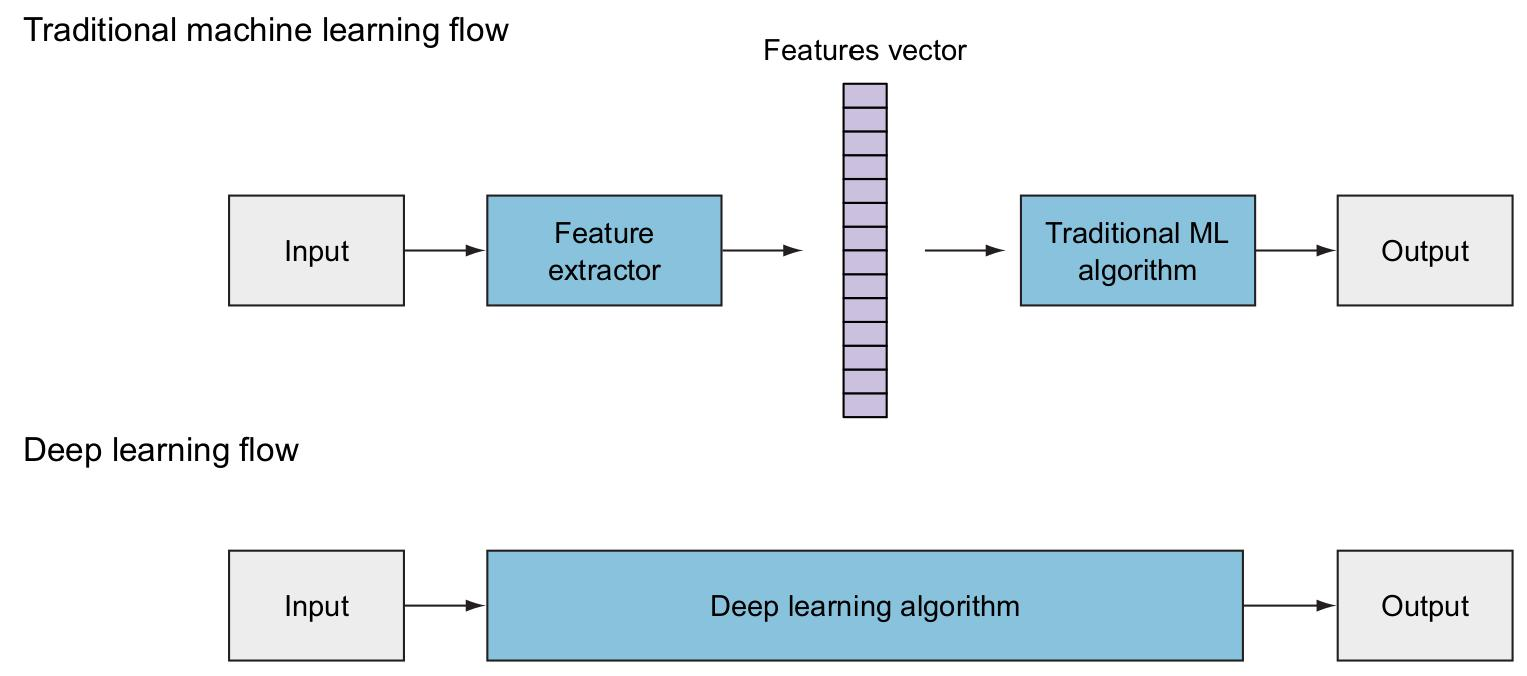
\includegraphics[scale=0.2]{images/traditional-vs-deep}
		\caption{Traditional ML algorithms require manual feature extraction. A deep neural network automatically extracts features by passing the input image through its layers.}
	\end{figure}
\end{frame}

\section{Perceptron}
\begin{frame}{Artificial Neural Network (ANN)}
	\begin{figure}[ht]
	\centering
	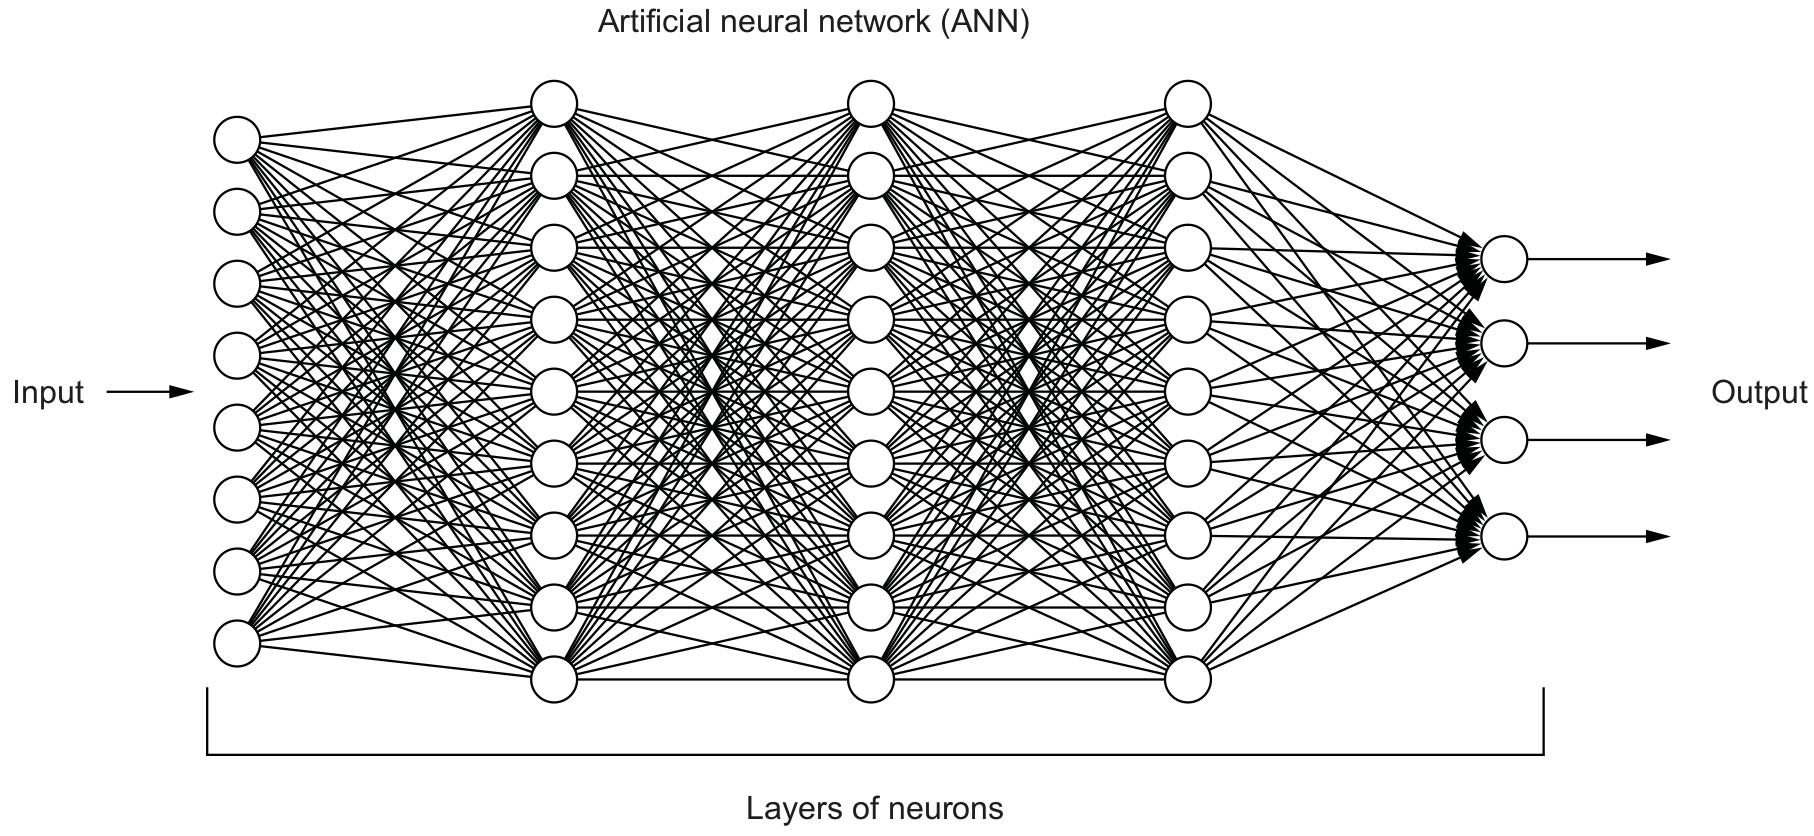
\includegraphics[scale=0.18]{images/anns}
	\caption{An artificial neural network consists of layers of nodes, or neurons connected with edges.}
\end{figure}	
\end{frame}


\begin{frame}{Perceptron}
	\begin{figure}[ht]
		\centering
		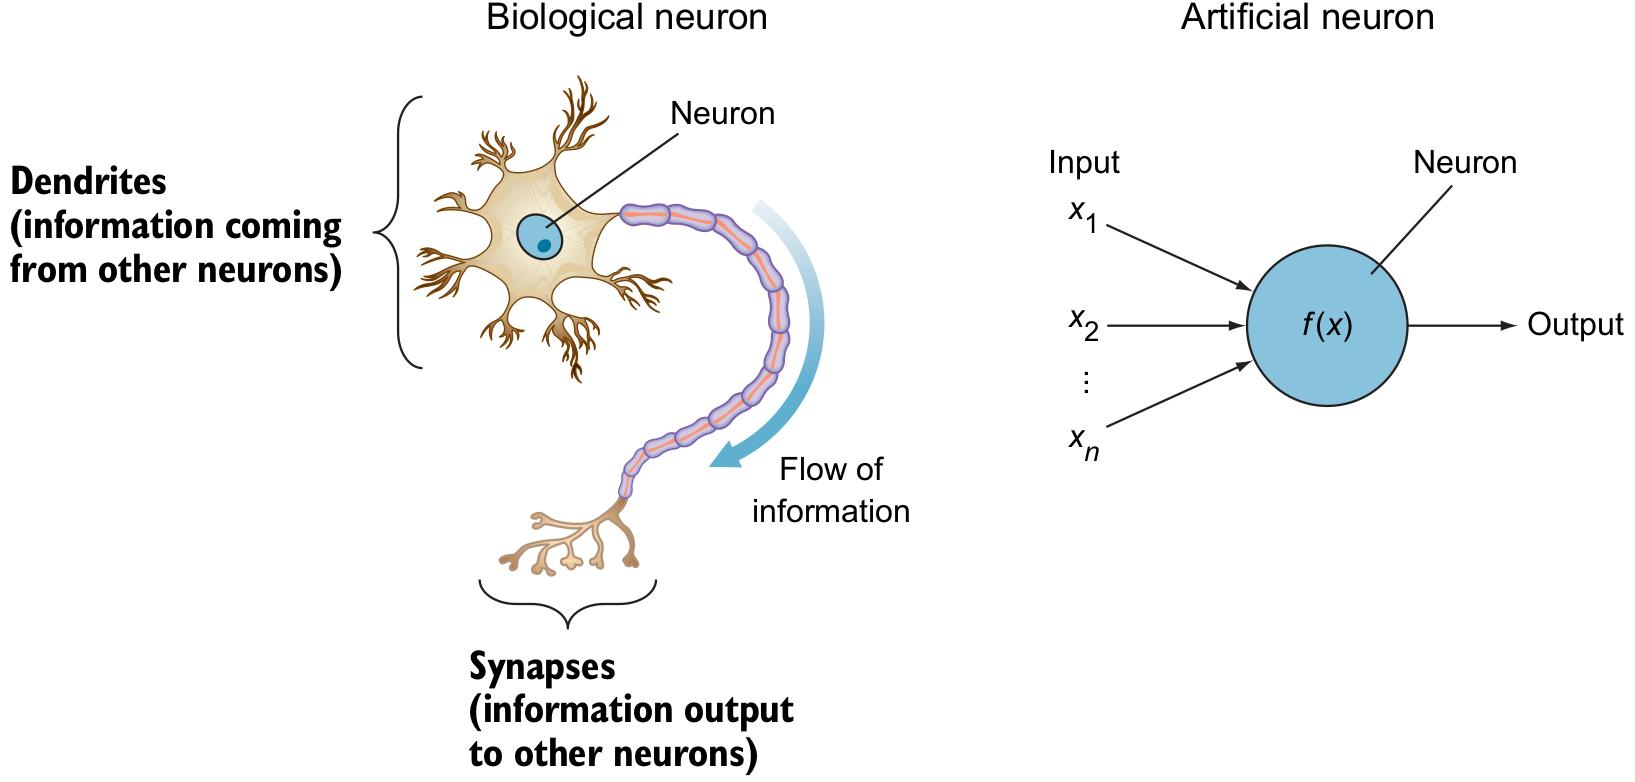
\includegraphics[scale=0.2]{images/ann}
		\caption{Artificial neurons were inspired by biological neurons. Different neurons are connected to each other by synapses that carry information.}
	\end{figure}	
\end{frame}

\begin{frame}{Calculation of a Neuron}
	\begin{figure}[ht]
		\centering
		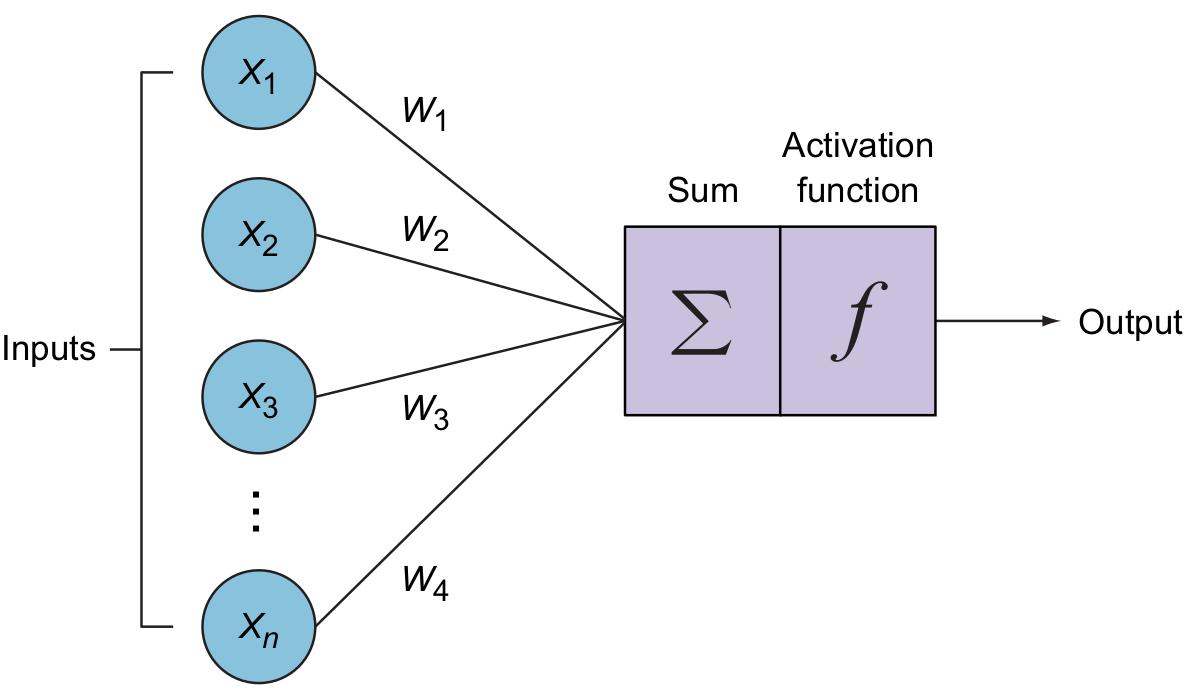
\includegraphics[scale=0.2]{images/calculation-perceptron}
		\caption{Input vectors are fed to the neuron, with weights assigned to represent importance. Calculations performed within the neuron are weighted sum and activation functions.}
	\end{figure}	
\end{frame}

\begin{frame}[fragile]{Weighted Sum Function}
	Weighted Sum Function dikenal juga sebagai kombinasi linier yang dituliskan sbb:
	\begin{align*}
		z &= \sum_{i=1}^n{x_1 \cdot w_i + b (\text{bias})}  \\
		  &= x_1 \cdot w_1 + x_2 \cdot w_2 + x_3 \cdot w_3 + \cdots + x_n \cdot w_n + b
	\end{align*}
	Dalam Python:
	\begin{minted}{python}
	z = np.dot(w.T, X) + b
	\end{minted}
\end{frame}

\begin{frame}{Bias dalam Perceptron}
	\begin{figure}[ht]
	\centering
	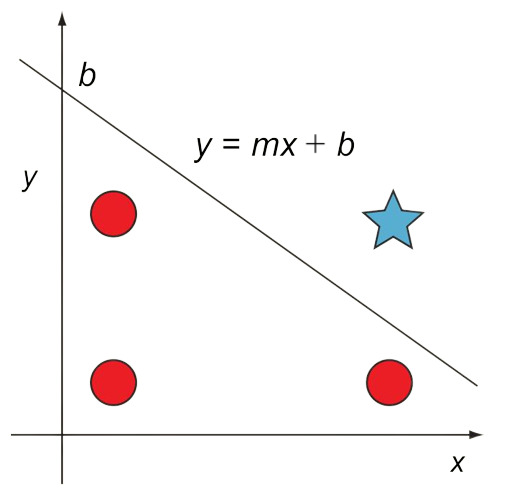
\includegraphics[scale=0.35]{images/persamaan-garis}
	\caption{Persamaan garis}
\end{figure}		
\end{frame}

\begin{frame}{Perceptron}
	\begin{figure}[ht]
		\centering
		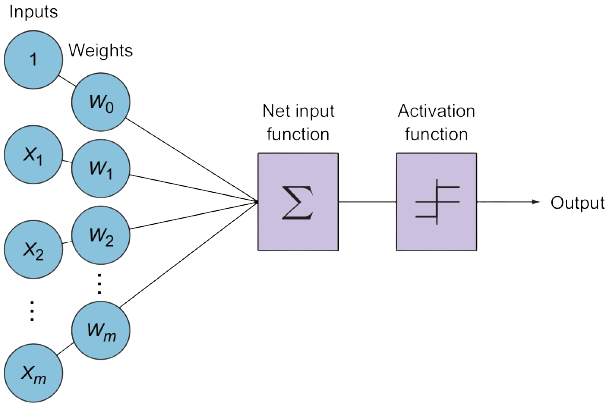
\includegraphics[scale=0.4]{images/perceptron}
		\caption{The input layer can be given biases by introducing an extra input that always has a value of 1.}
	\end{figure}		
\end{frame}

\begin{frame}{Step Activation Function (1/3)}
	\begin{itemize}
		\item<2-> Activation function mempunyai banyak bentuk. 
		\item<3-> Salah satu activation function adalah \textbf{step activation function}.
	\end{itemize}
\end{frame}

\begin{frame}{Step Activation Function (2/3)}
	\begin{figure}[ht]
	\centering
	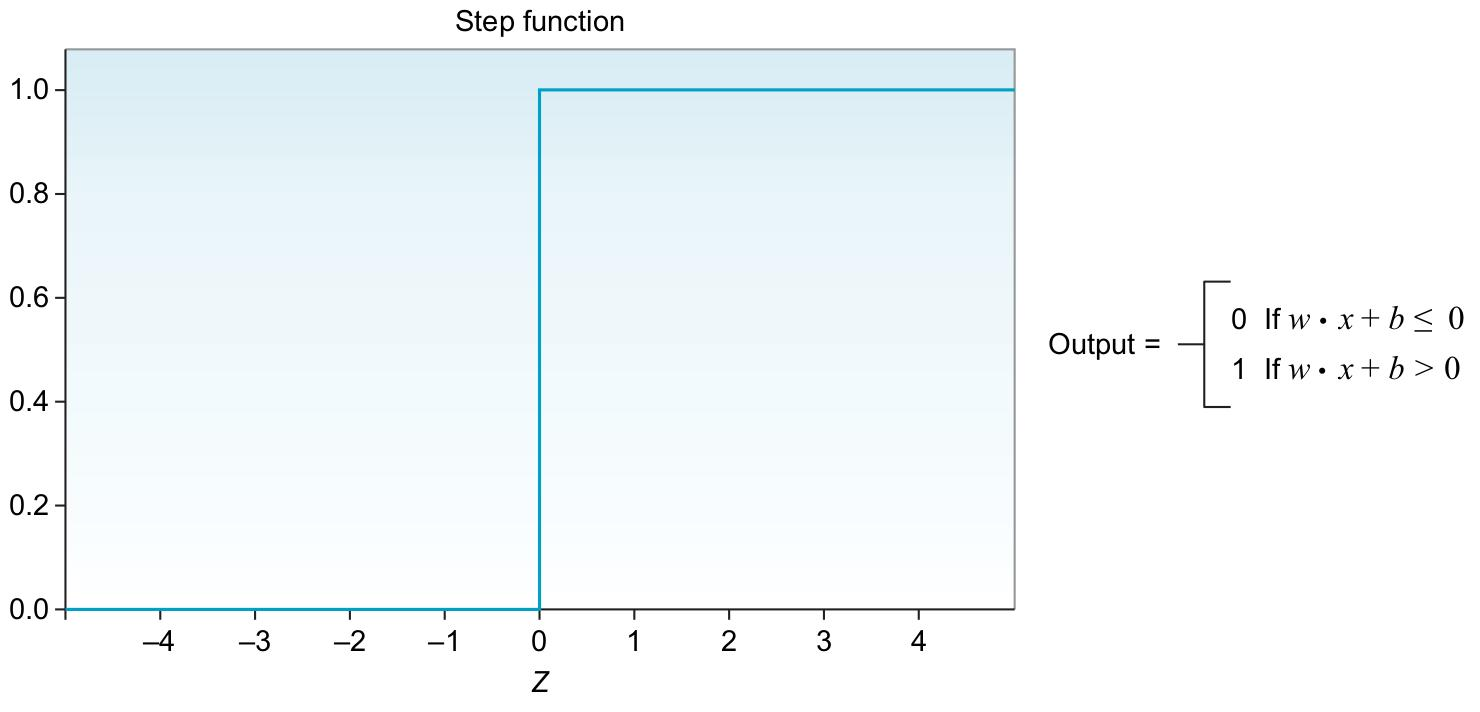
\includegraphics[scale=0.2]{images/step-activation-function}
	\caption{The step function produces a binary output (\texttt{0} or \texttt{1}). If the summed input $\geq$ \texttt{0}, it "fires" (\texttt{output = 1}); else (\texttt{summed input < 0}) it doesn't fire (\texttt{output = 0})}
\end{figure}			
\end{frame}

\begin{frame}[fragile]{Step Activation Function (3/3)}
	Dalam Python:
	\begin{minted}{python}
def step_function(z):
    if z <= 0:
        return 0
    else:
        return 1
	\end{minted}
\end{frame}

\begin{frame}{How does the Perceptron Learn? (1/2)}
	\begin{figure}[ht]
	\centering
	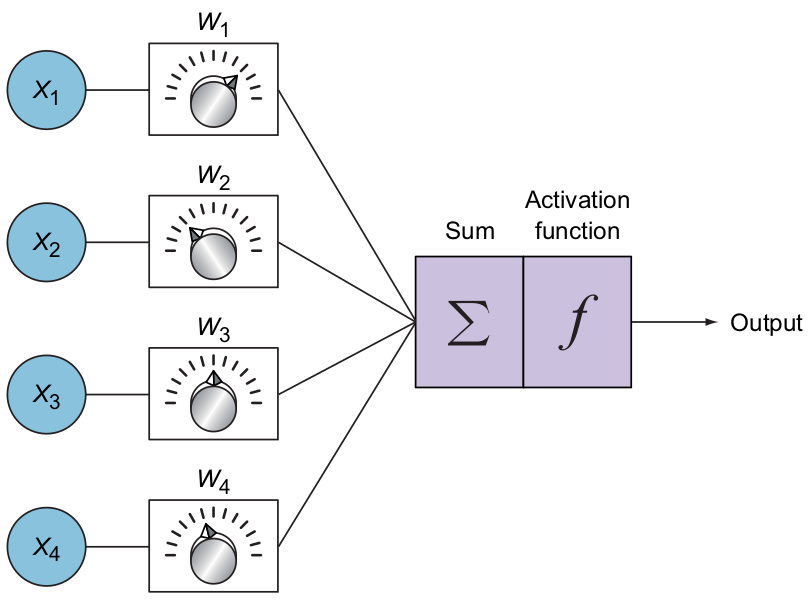
\includegraphics[scale=0.25]{images/perceptron-how}
	\caption{Weights are tuned up and down during the learning process to optimize the value of the loss function}
\end{figure}				
\end{frame}

\begin{frame}{How does the Perceptron Learn? (2/2)}
	\begin{enumerate}
		\item<2-> The neuron calculates the weighted sum and applies the activation function to make a prediction $\hat{y}$. Ini disebut \textbf{feedforward process}:
		\begin{equation*}
			\hat{y} = \text{activation}\left( \sum{x_1 \cdot w_i + b} \right)
		\end{equation*}
		\item<3-> It compares the output prediction with the correct label to calculate the error:
		\begin{equation*}
			\text{error} = y - \hat{y}
		\end{equation*}
		\item<4-> It then updates the weight. If the prediction is too high, it adjusts the weight to make a lower prediction the next time, and vice versa.
		\item<5-> Repeat!
	\end{enumerate}
\end{frame}

\begin{frame}{Is One Neuron Enough to Solve Complex Problems? (1/2)}
	The answer is no. The perceptron is a linear function.
	\begin{figure}[ht]
	\centering
	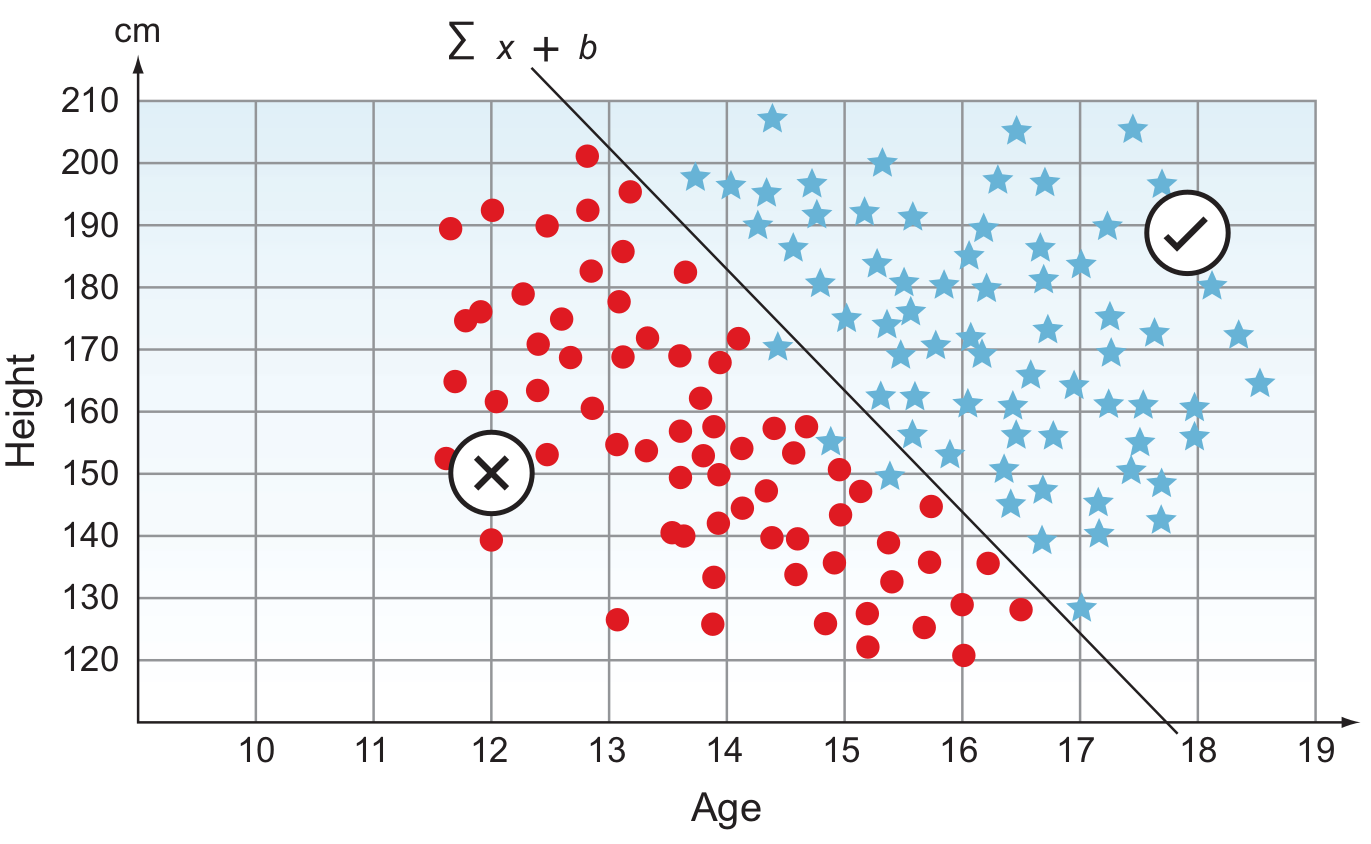
\includegraphics[scale=0.2]{images/linear-separable}
	\caption{Linearly separable data can be separated by a straight line}
\end{figure}					
\end{frame}

\begin{frame}{Is One Neuron Enough to Solve Complex Problems? (2/2)}
	\begin{figure}[ht]
		\centering
		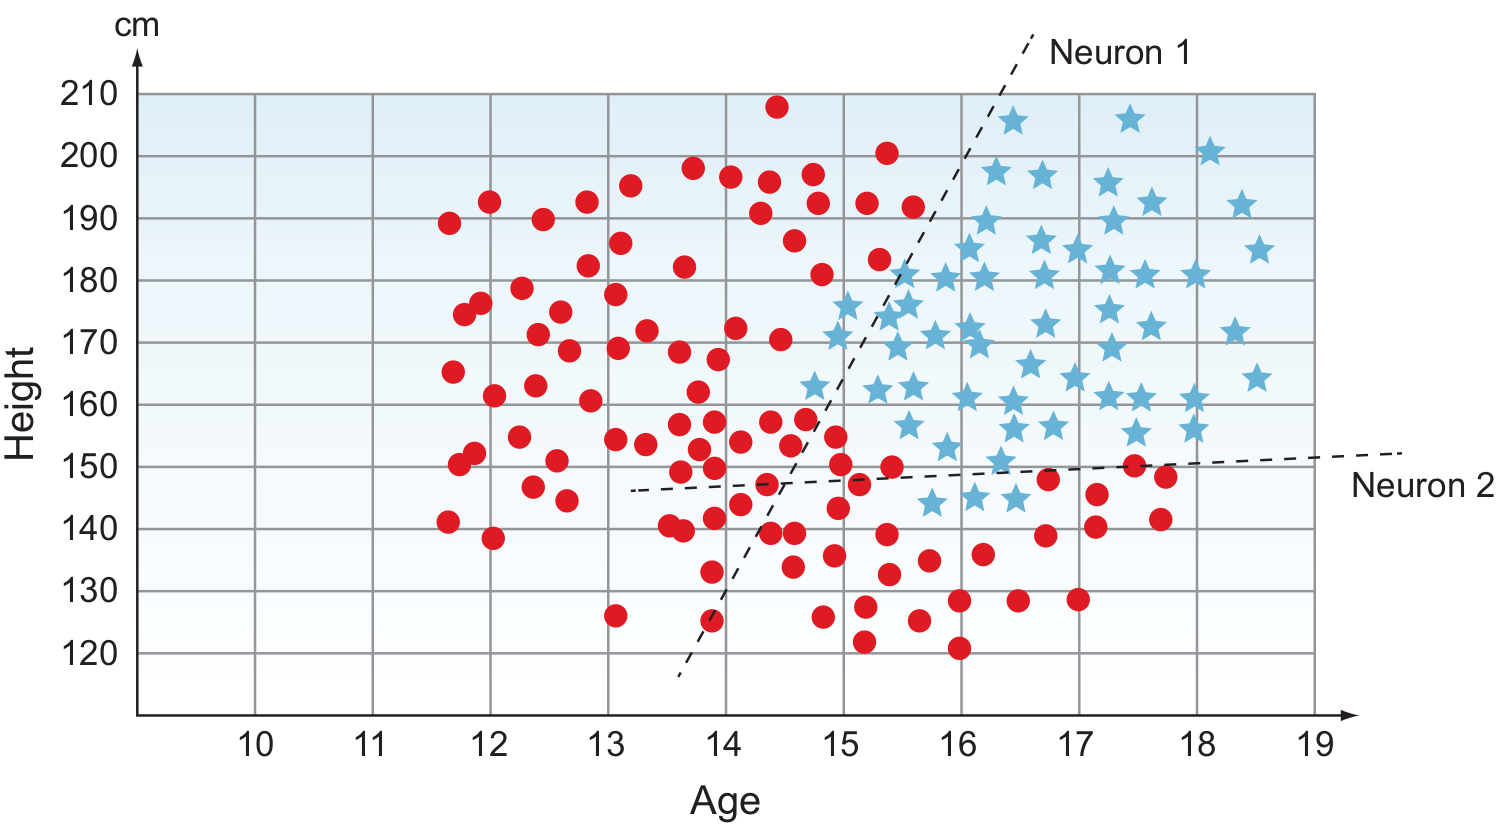
\includegraphics[scale=0.2]{images/nonlinear-separable}
		\caption{In a nonlinear dataset, a single straight line cannot separate the training data. A network with two perceptrons can produce two lines and help separate the data further in this example.}
	\end{figure}					
\end{frame}

\section{Multilayer Perceptrons}
\begin{frame}{Multilayer Perceptrons (1/3)}
	Single perceptron works great with simple datasets that can be separated by a line tetapi real world jauh lebih kompleks daripada itu.
	
	\begin{itemize}
		\item<2-> Linear datasets---The data can be split with a single straight line. 
		\item<3-> Nonlinear datasets---The data cannot be split with a single straight line. We need more than one line to form a shape that splits the data.
	\end{itemize}
\end{frame}

\begin{frame}{Multilayer Perceptrons (2/3)}
	\begin{figure}[ht]
		\centering
		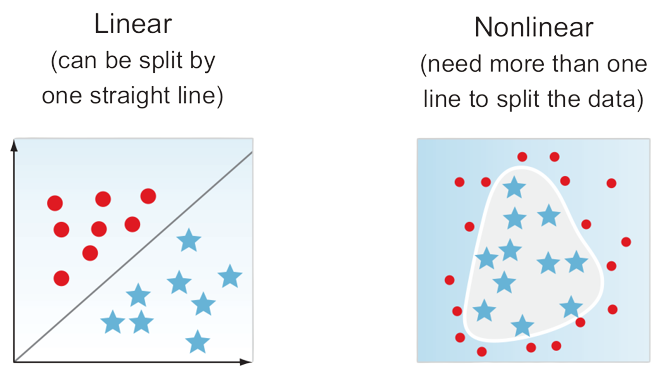
\includegraphics[scale=0.4]{images/linear-vs-nonlinear}
		\caption{Examples of linear data and nonlinear data}
	\end{figure}					
\end{frame}

\begin{frame}{Multilayer Perceptrons (3/3)}
	\begin{figure}[ht]
		\centering
		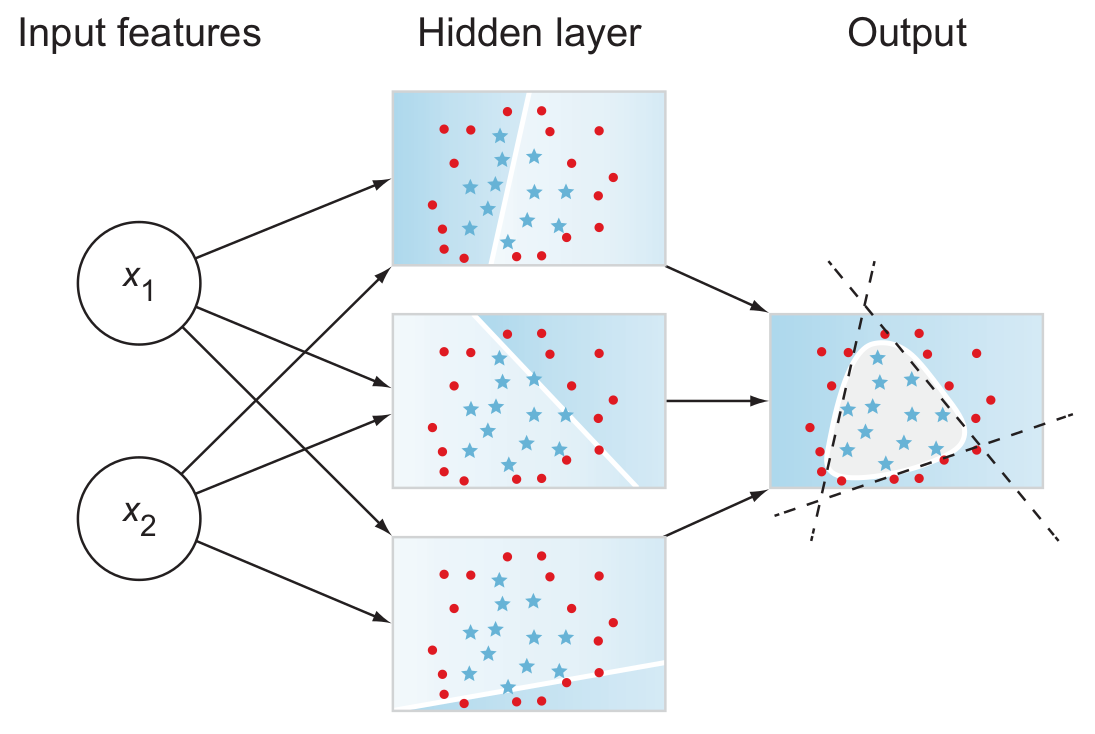
\includegraphics[scale=0.225]{images/multilayer-perceptrons}
		\caption{A perceptron is a linear function that produces a straight line. So to fit this data, we need three perceptrons to create a triangle-like shape that splits the dark dots.}
	\end{figure}					
\end{frame}

\begin{frame}{Multilayer Perceptron Architecture (1/)}
	\begin{figure}[ht]
		\centering
		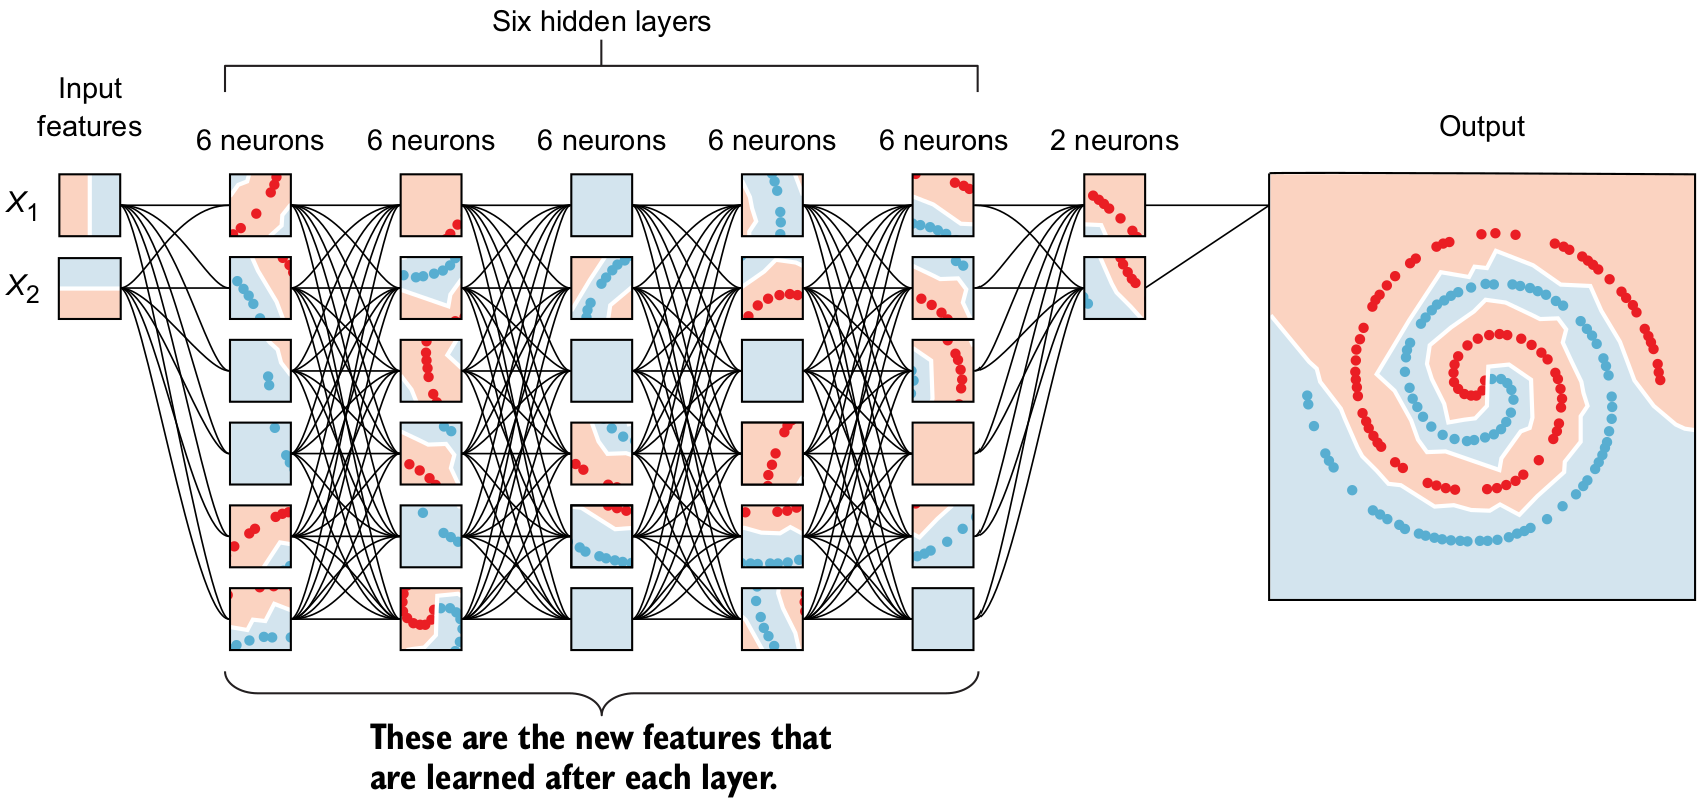
\includegraphics[scale=0.18]{images/tensorflow-playground}
		\caption{Tensorflow playground example representation of the feature learning in a deep neural network}
	\end{figure}					
\end{frame}

\begin{frame}{Multilayer Perceptron Architecture (2/)}
	The main components of the neural network architecture are as follows:
	\begin{itemize}
		\item<2-> Input layer
		\item<3-> Hidden layers
		\item<4-> Weight connections (edges) 
	\end{itemize}
\end{frame}

\begin{frame}{Fully Connected Layers (1/)}
	\begin{figure}[ht]
	\centering
	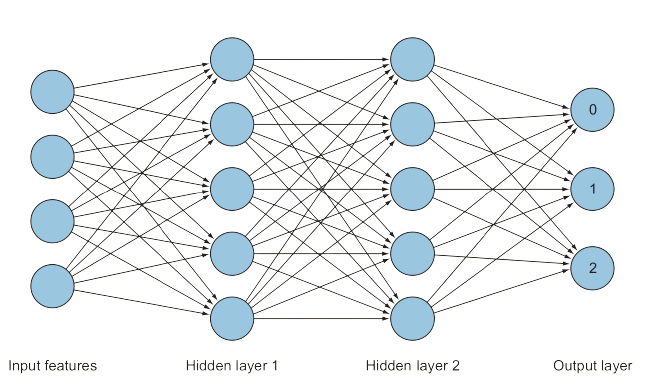
\includegraphics[scale=0.4]{images/fully-connected}
	\caption{A fully connected network}
\end{figure}						
Berapakah banyak parameter dari MLP ini?
\end{frame}

\begin{frame}{Neural Network Hyperparameters}
	\begin{itemize}
		\item<2-> Number of hidden layers
		\item<3-> Activation function
		\item<4-> Error function
		\item<5-> Optimizer
		\item<6-> Batch size
		\item<7-> Number of epochs
		\item<8-> Learning rate 
	\end{itemize}
\end{frame}

\section{Activation Functions}
\begin{frame}{Linear Transfer Function}
	\begin{figure}[ht]
	\centering
	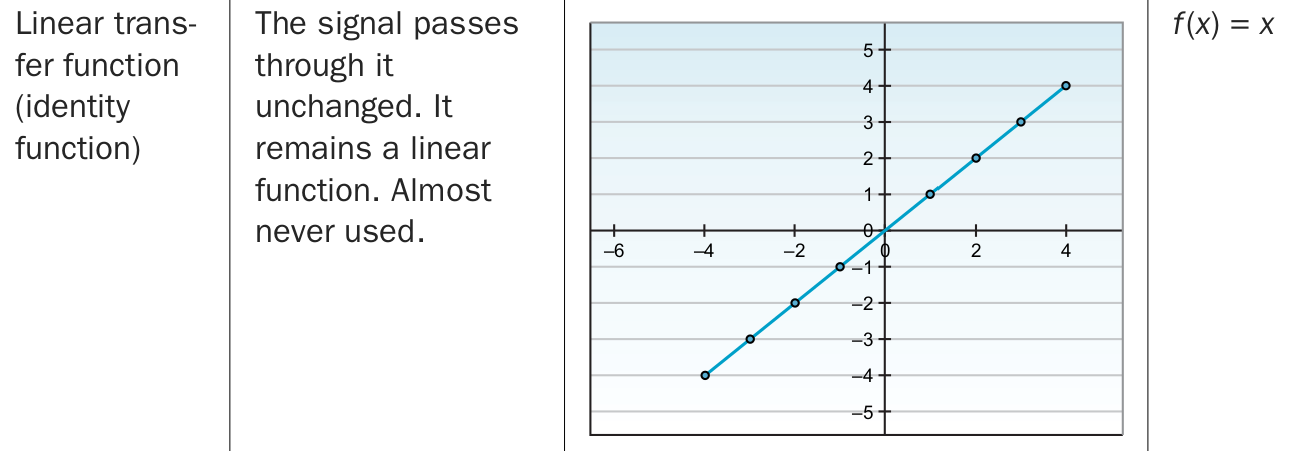
\includegraphics[scale=0.25]{images/linear-transformation}
\end{figure}							
\end{frame}

\begin{frame}{Heaviside Step Function}
	\begin{figure}[ht]
		\centering
		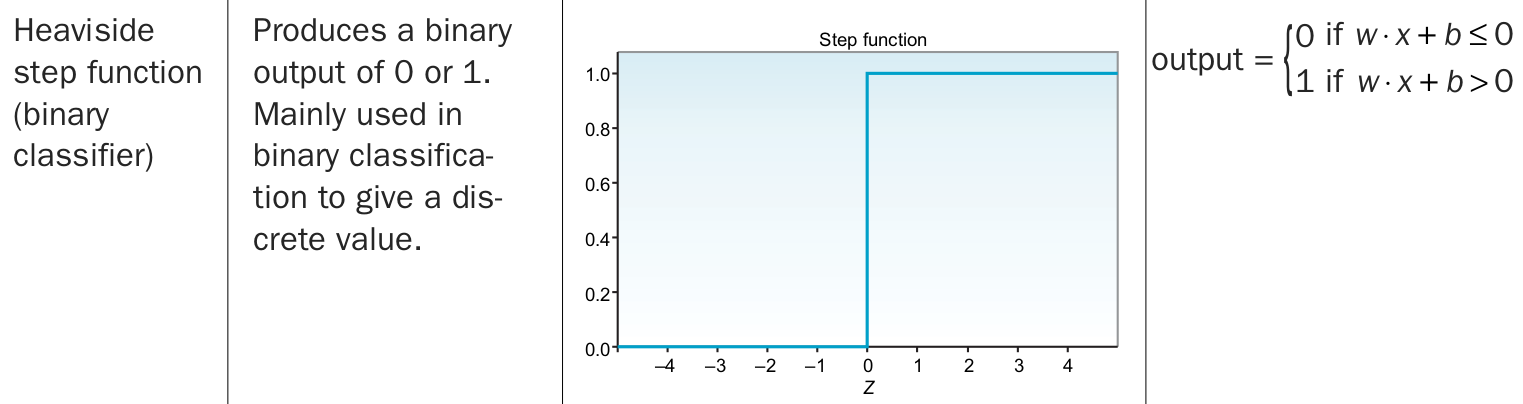
\includegraphics[scale=0.2]{images/heaviside-step-function}
	\end{figure}							
\end{frame}

\begin{frame}{Sigmoid/Logistic Function}
	\begin{figure}[ht]
		\centering
		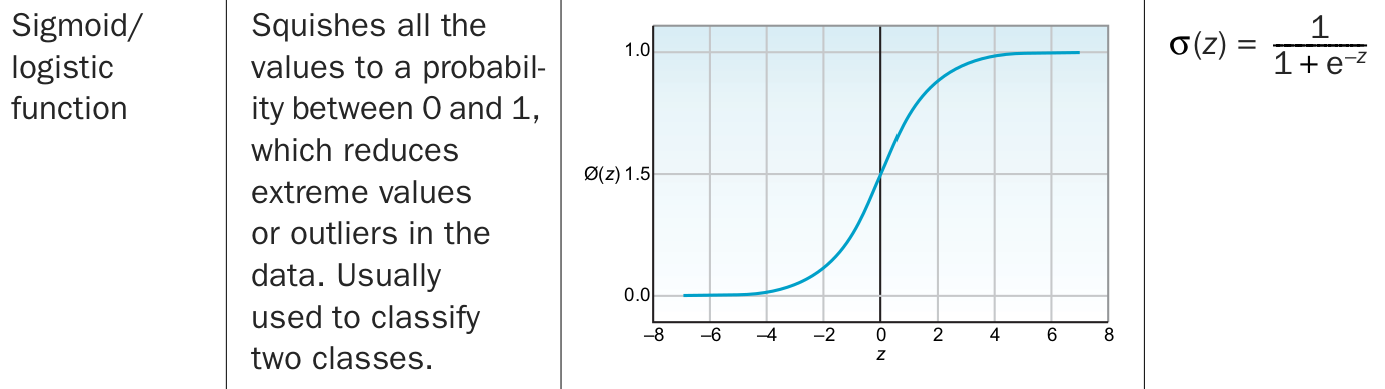
\includegraphics[scale=0.2]{images/sigmoid-function}
	\end{figure}							
\end{frame}

\begin{frame}{Softmax Function}
	\begin{figure}[ht]
		\centering
		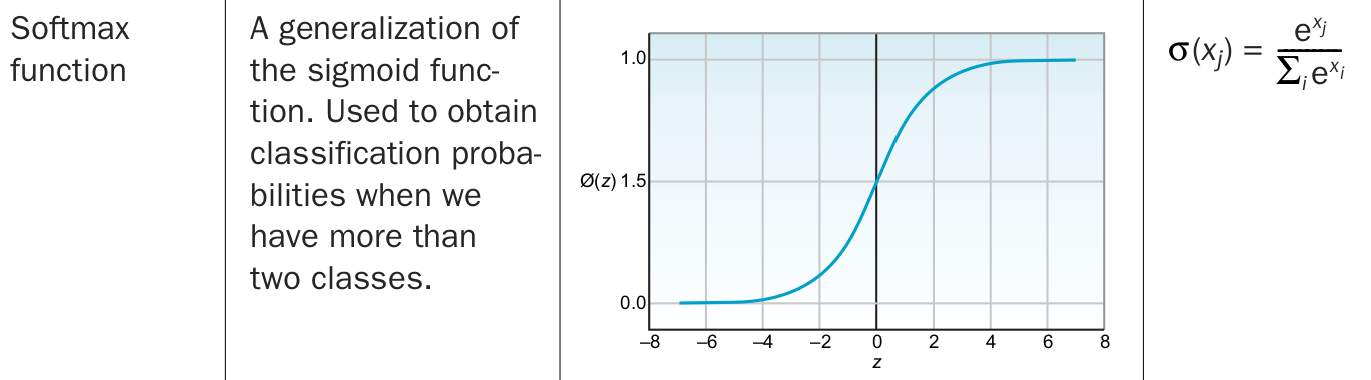
\includegraphics[scale=0.2]{images/softmax-function}
	\end{figure}							
\end{frame}

\begin{frame}{Hyperbolic Tangent Function}
	\begin{figure}[ht]
		\centering
		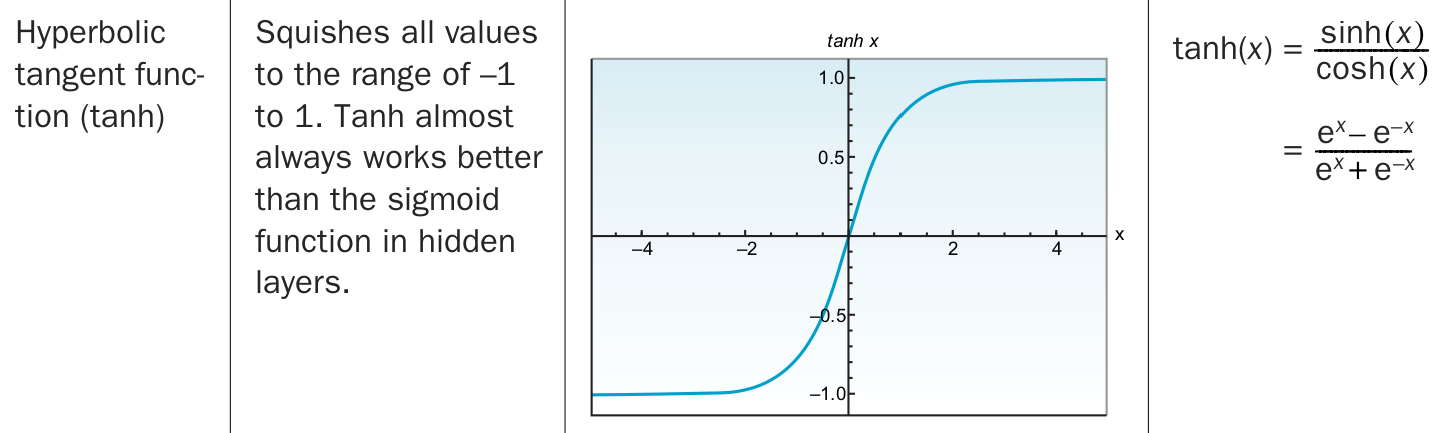
\includegraphics[scale=0.2]{images/tanh-function}
	\end{figure}							
\end{frame}

\begin{frame}{Rectified Linear Unit}
	\begin{figure}[ht]
		\centering
		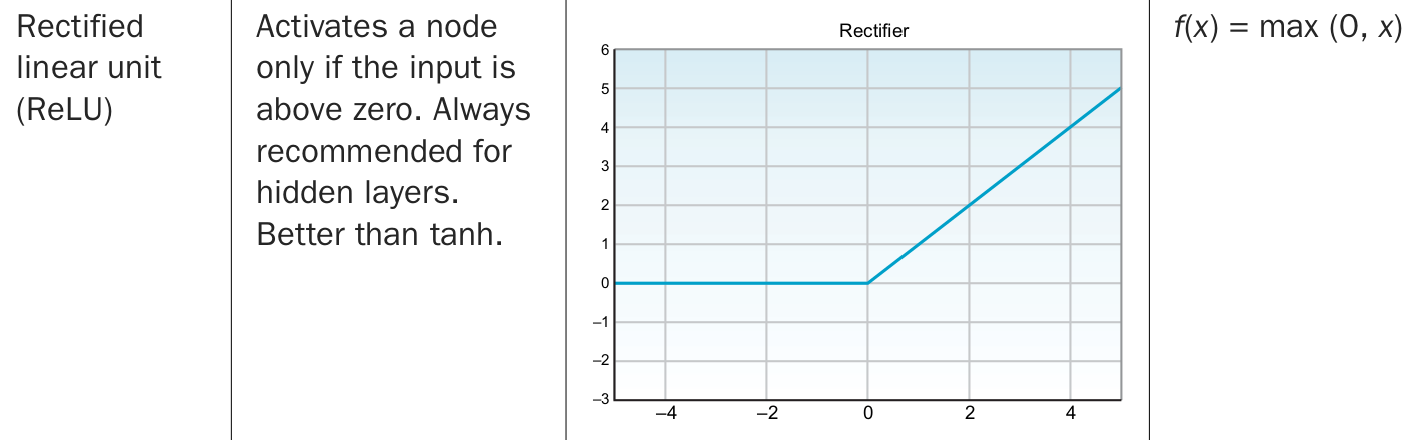
\includegraphics[scale=0.2]{images/relu-function}
	\end{figure}							
\end{frame}

\begin{frame}{Leaky ReLU}
	\begin{figure}[ht]
		\centering
		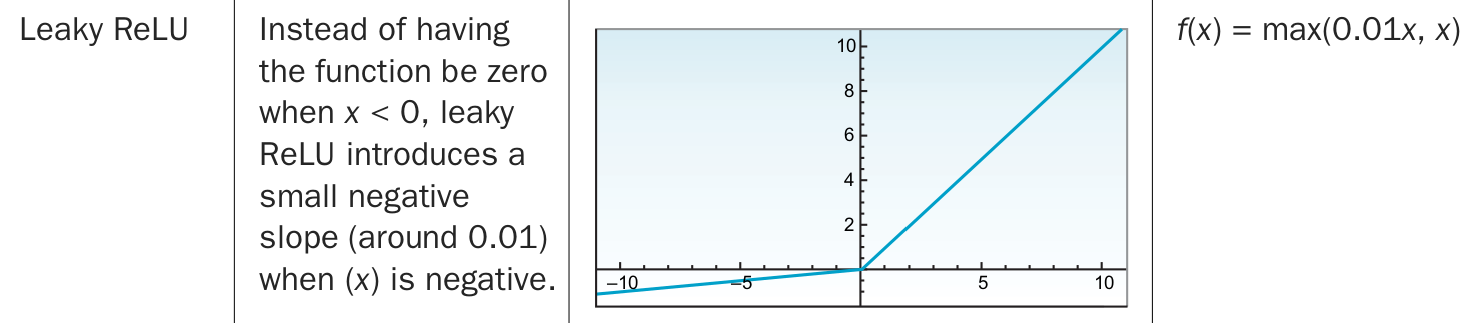
\includegraphics[scale=0.2]{images/leaky-function}
	\end{figure}							
\end{frame}

\begin{frame}{Hyperparameter Alert}
	\begin{itemize}
		\item<2-> For hidden layers---In most cases, you can use the ReLU activation function (or leaky ReLU) in hidden layers.
		\item<3-> For the output layer
		\begin{itemize}
			 \item<4-> The softmax activation function $\rightarrow$ most classification problems when the classes are mutually exclusive. 
			 \item<5-> The sigmoid function $\rightarrow$ binary classification. 
			 \item<6-> For regression problems $\rightarrow$ no activation function.
		\end{itemize}	 
	\end{itemize}
\end{frame}

\begin{frame}{A Simple Three-layer Neural Network}
	\begin{figure}[ht]
		\centering
		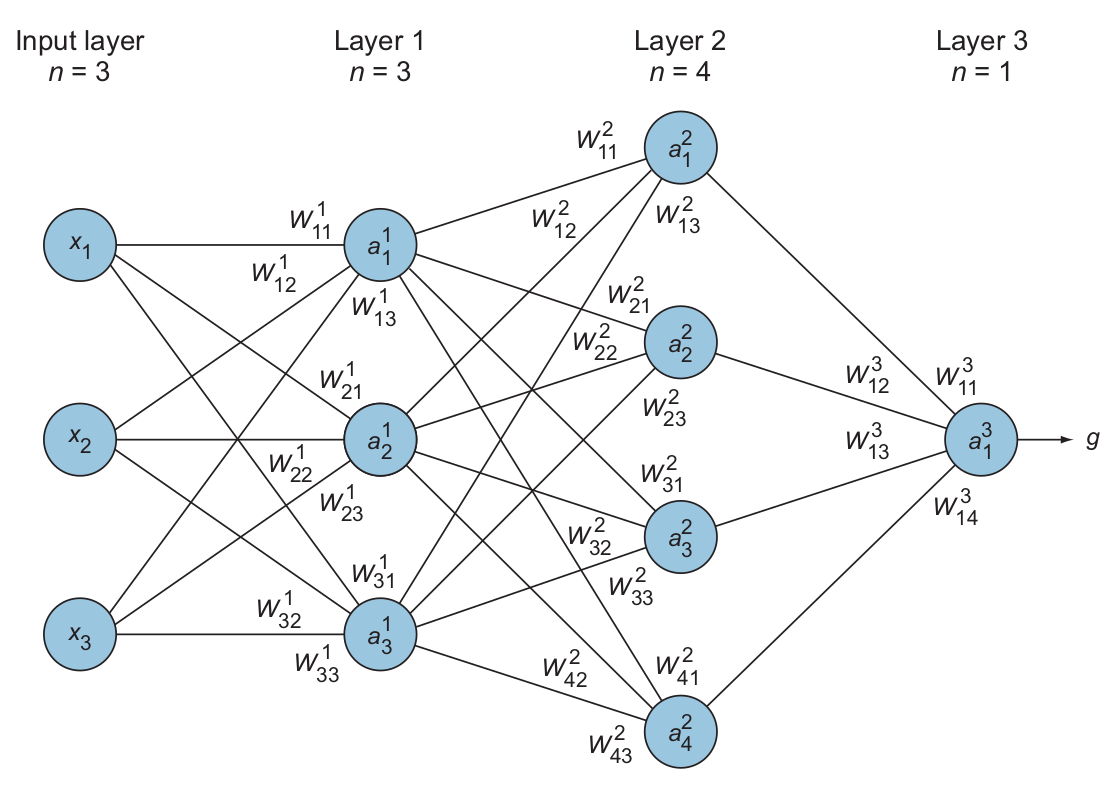
\includegraphics[scale=0.25]{images/simple-neural-network}
		\caption{A simple three-layer neural network}
	\end{figure}							
\end{frame}

\begin{frame}{Feedforward Calculations}
	Pada layer 1,
	\begin{align*}
		a_1^{(1)} &= \sigma(w_{11}^{(1)} x_1 + w_{21}^{(1)} x_2 + w_{31}^{(1)} x_3)  \\
		a_2^{(1)} &= \sigma(w_{12}^{(1)} x_1 + w_{22}^{(1)} x_2 + w_{32}^{(1)} x_3)  \\
		a_3^{(1)} &= \sigma(w_{13}^{(1)} x_1 + w_{23}^{(1)} x_2 + w_{33}^{(1)} x_3) 
	\end{align*}
	\onslide<2-> Lakukan perhitungan yang sama pada layer 2,
	\begin{equation*}
		\onslide<3-> a_1^{(2)}, a_2^{(2)}, a_3^{(2)} \text{ dan }a_4^{(2)}.
	\end{equation*}
	Hasil prediksi di layer 3 adalah
	\begin{equation*}
		\hat{y} = a_1^{(2)} = \sigma( w_{11}^{(3)} a_1^{(2)} + w_{12}^{(3)} a_2^{(2)} + w_{13}^{(3)} a_3^{(2)} + w_{14}^{(3)} a_4^{(2)} )
	\end{equation*}
\end{frame}

\begin{frame}{Feedforward Calculations (versi Matriks)}
	\begin{equation*}
		\hat{y} = \sigma \cdot W^{(3)} \cdot \sigma \cdot W^{(2)} \cdot \sigma \cdot W^{(1)} \cdot (x). 
	\end{equation*}
	\begin{figure}[ht]
	\centering
	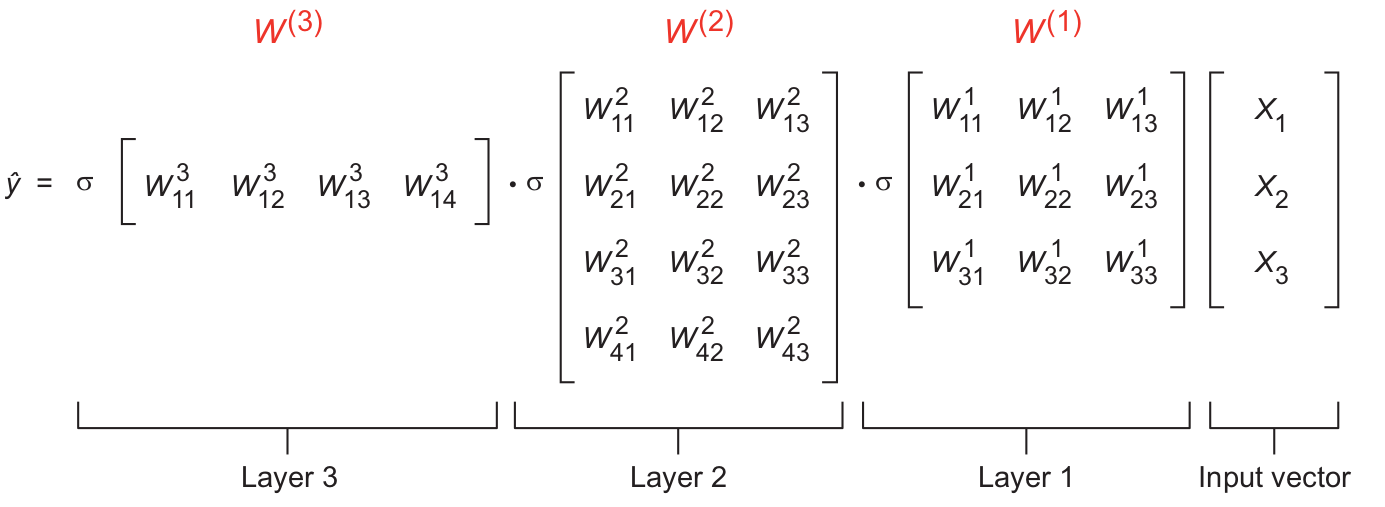
\includegraphics[scale=0.2]{images/feedforward-matriks}
	\caption{Reading from left to right, we stack the inputs together in one vector, multiply the input vector by the weights matrix from layer 1, apply the sigmoid function, and multiply the result}
\end{figure}							
\end{frame}

\begin{frame}{Feature Learning (1/2)}
	\begin{figure}[ht]
	\centering
	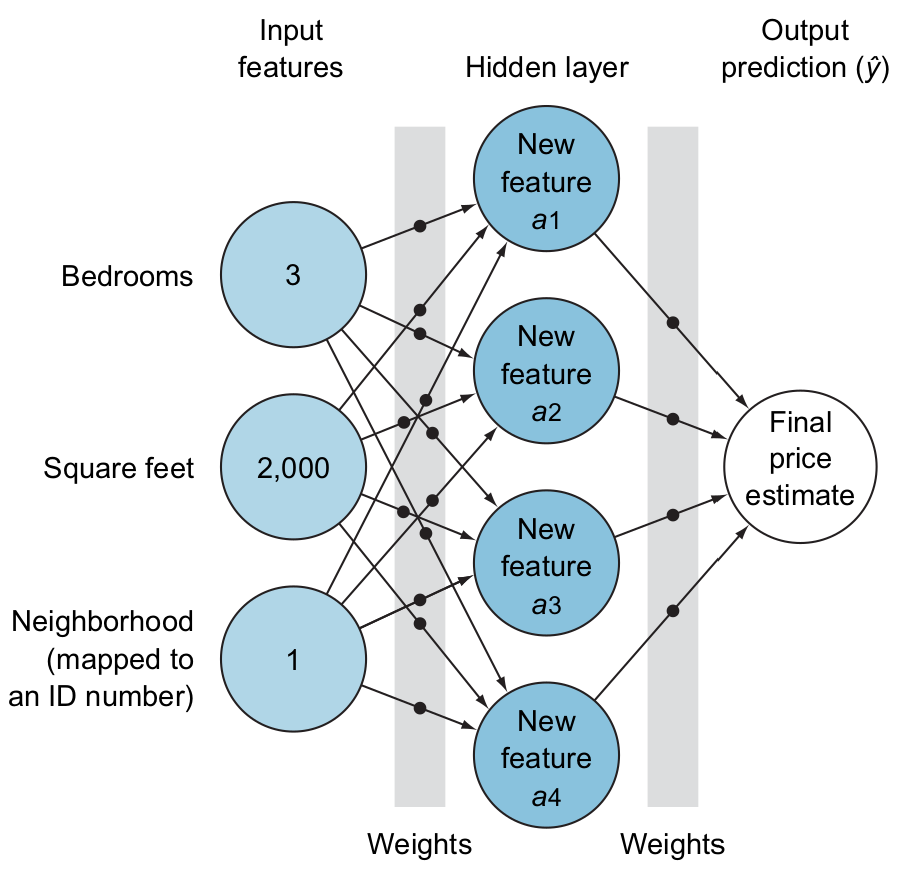
\includegraphics[scale=0.2]{images/small-network}
	\caption{A small neural network to estimate the price of a house based on three features: how many bedrooms it has, how big it is, and which neighborhood it is in}
\end{figure}								
\end{frame}

\begin{frame}{Feature Learning (2/2)}
	\begin{figure}[ht]
		\centering
		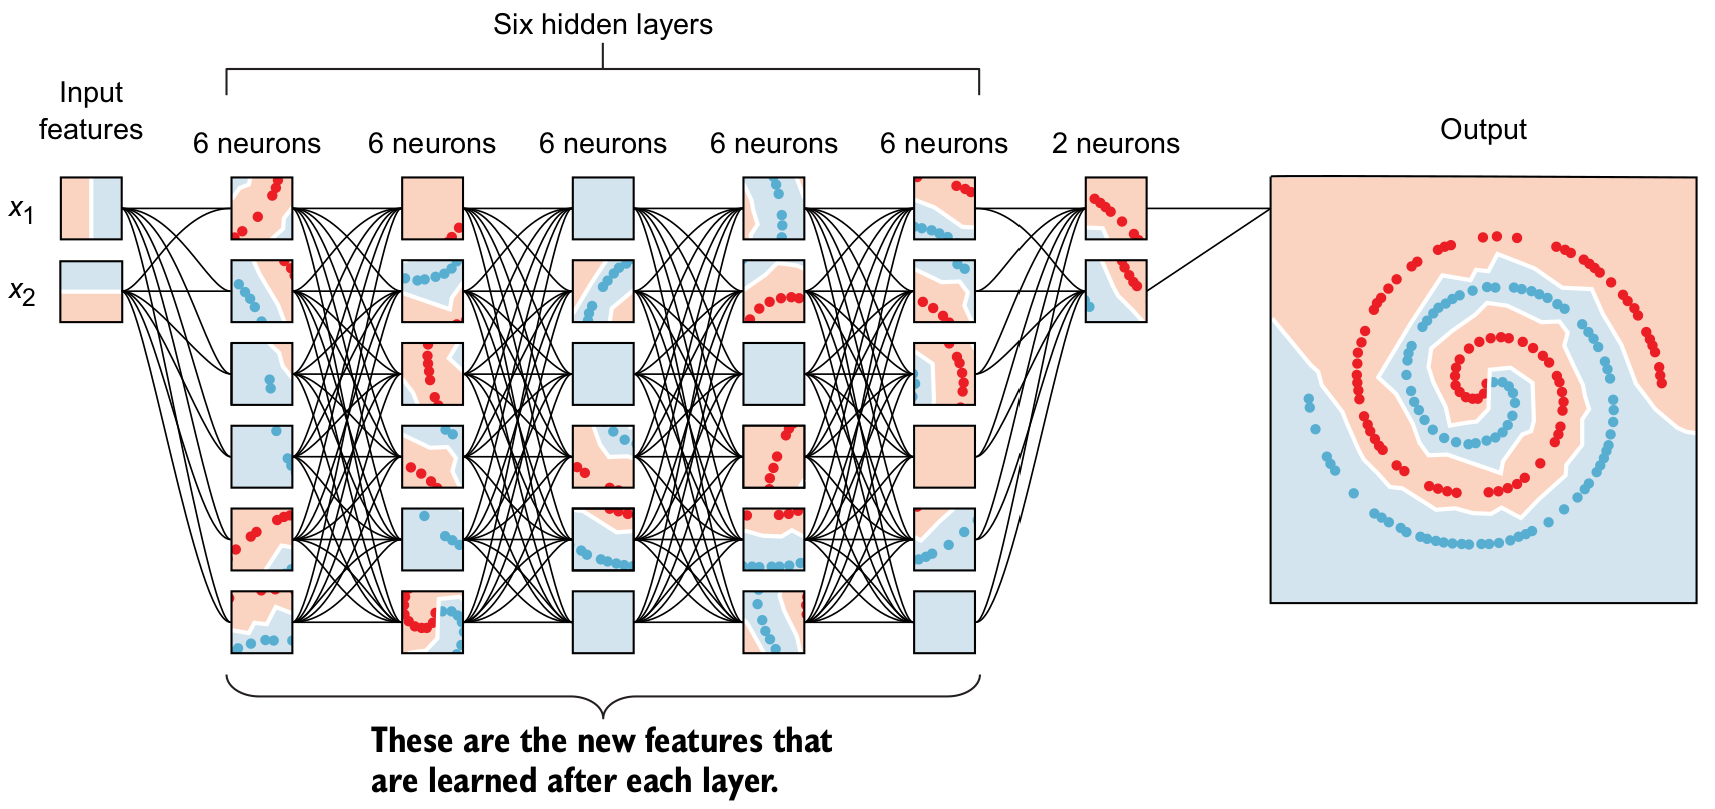
\includegraphics[scale=0.19]{images/feature-learning}
		\caption{Learning features in multiple hidden layers}
	\end{figure}								
\end{frame}

\begin{frame}{Loss Functions}
	\begin{figure}[ht]
		\centering
		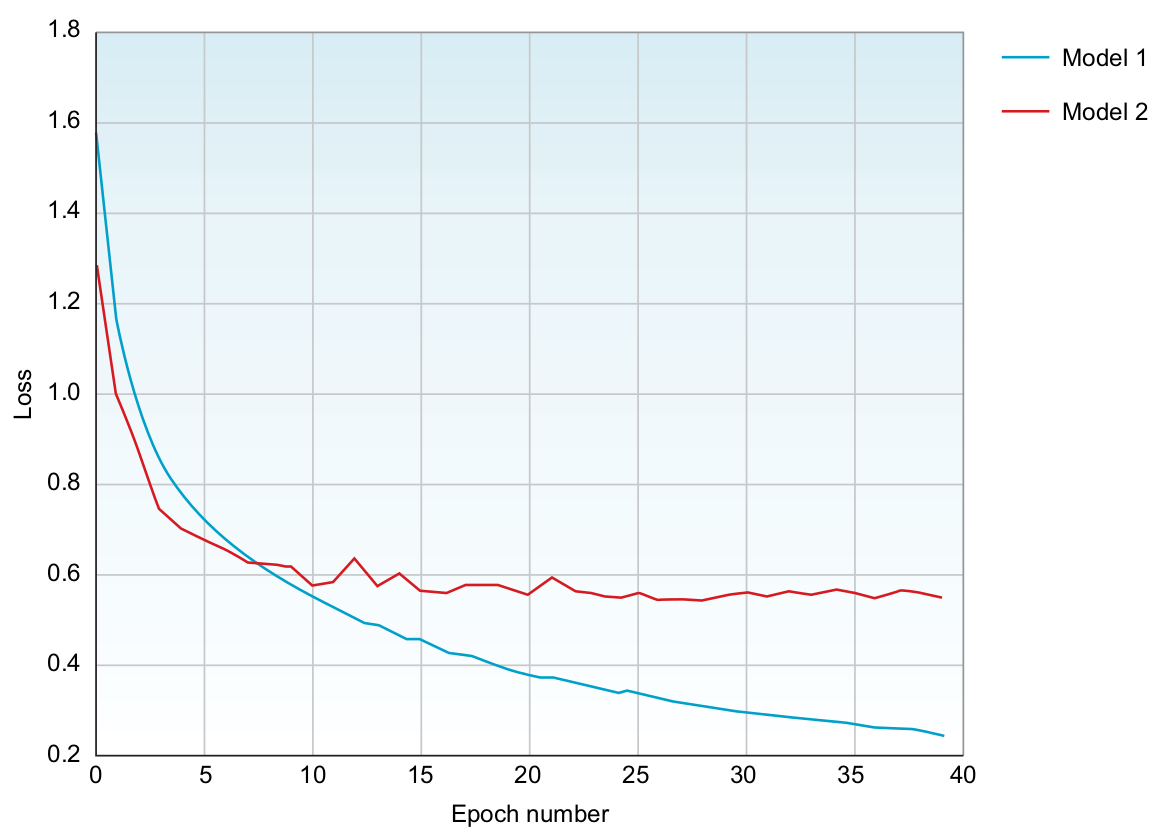
\includegraphics[scale=0.2]{images/loss-functions}
		\caption{A visualization of the loss functions of two separate models plotted over time}
	\end{figure}								
	\onslide<2-> Model manakah yang lebih baik?
\end{frame}

\begin{frame}{Mean Square Error}
	Mean squared error (MSE) is commonly used in regression problems that require the output to be a real value (like house pricing).
	\begin{equation*}
		E(W,b) = \frac{1}{N} \sum_{i=1}^N{(\hat{y}_i - y_i)^2}.
	\end{equation*}
	Variasi lain dari MSE adalah \textit{mean absolute error} (MAE), yaitu:
	\begin{equation*}
	E(W,b) = \frac{1}{N} \sum_{i=1}^N{\left| \hat{y}_i - y_i \right| }.
	\end{equation*}
\end{frame}

\begin{frame}{Penjelasan Notasi}
	\begin{figure}[ht]
	\centering
	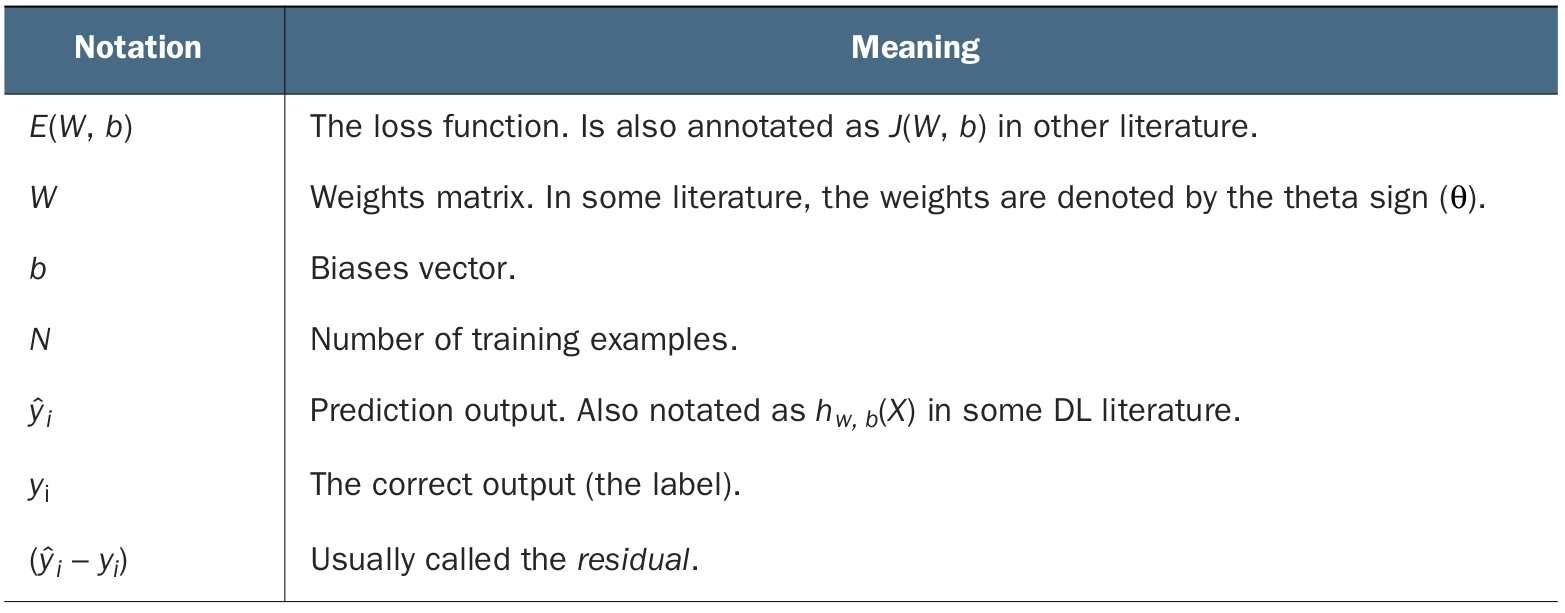
\includegraphics[scale=0.2]{images/notation}
	\caption{Meanings of notation used in regression problems}
\end{figure}								
\end{frame}

\begin{frame}{Cross-entropy}
	Cross-entropy is commonly used in classification problems because it quantifies the difference between two probability distributions.
	\begin{equation*}
		E(W,b) = -\sum_{i=1}^m{ \hat{y}_i \log(p_i) }
	\end{equation*}
	To calculate the cross-entropy error across all the training examples ($n$), we use this general formula: 
	\begin{equation*}
		E(W,b) = -\sum_{i=1}^n \sum_{i=1}^m{ \hat{y}_{ij} \log( p_{ij} ) }
	\end{equation*}
\end{frame}

\begin{frame}{Algoritma Optimasi (1/3)}
	\begin{figure}[ht]
	\centering
	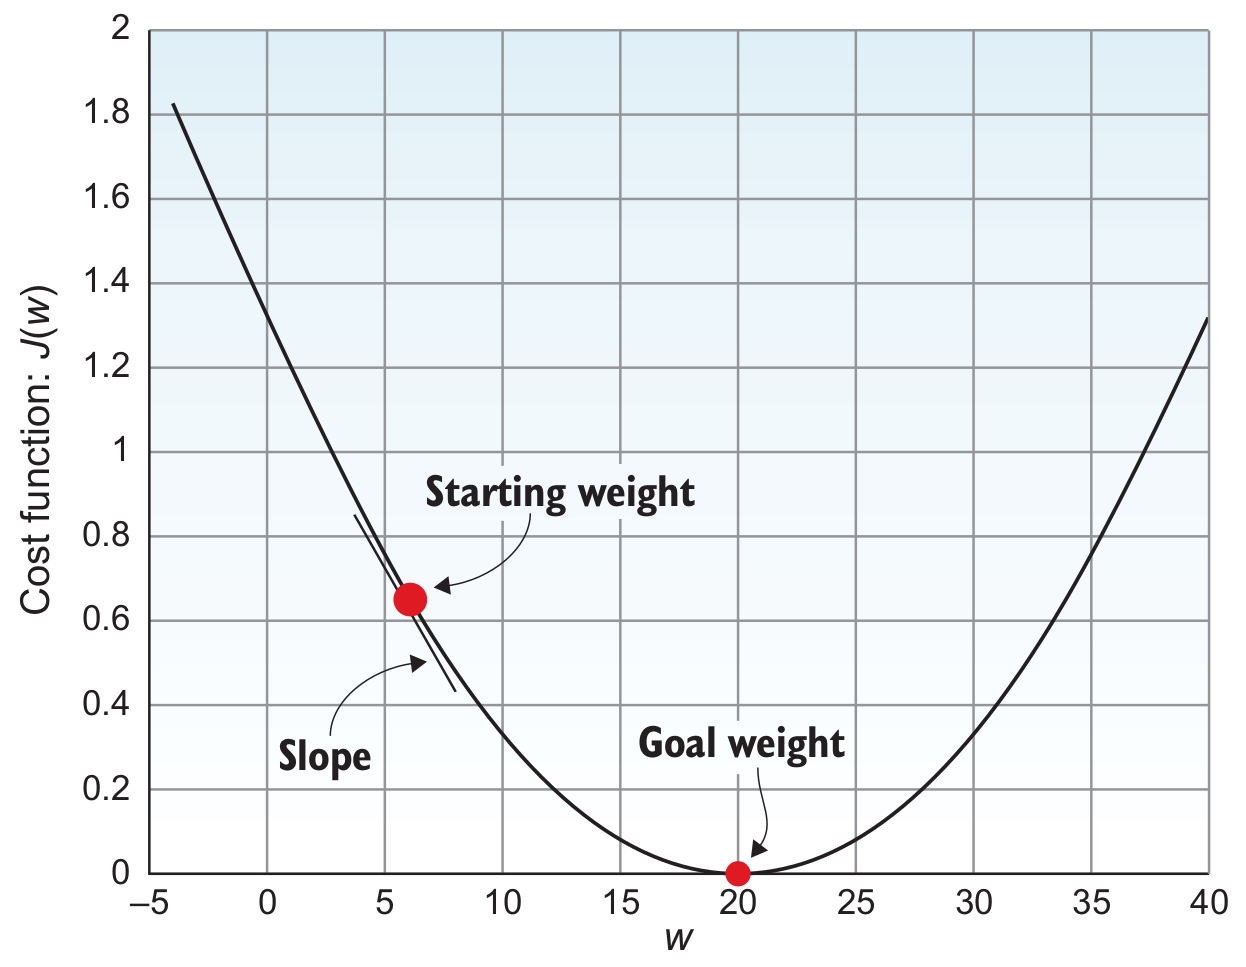
\includegraphics[scale=0.2]{images/cost-function}
	\caption{The error function with respect to its weight for a single perceptron is a 2D curve}
\end{figure}									
\end{frame}

\begin{frame}{Algoritma Optimasi (2/3)}
	\begin{figure}[ht]
		\centering
		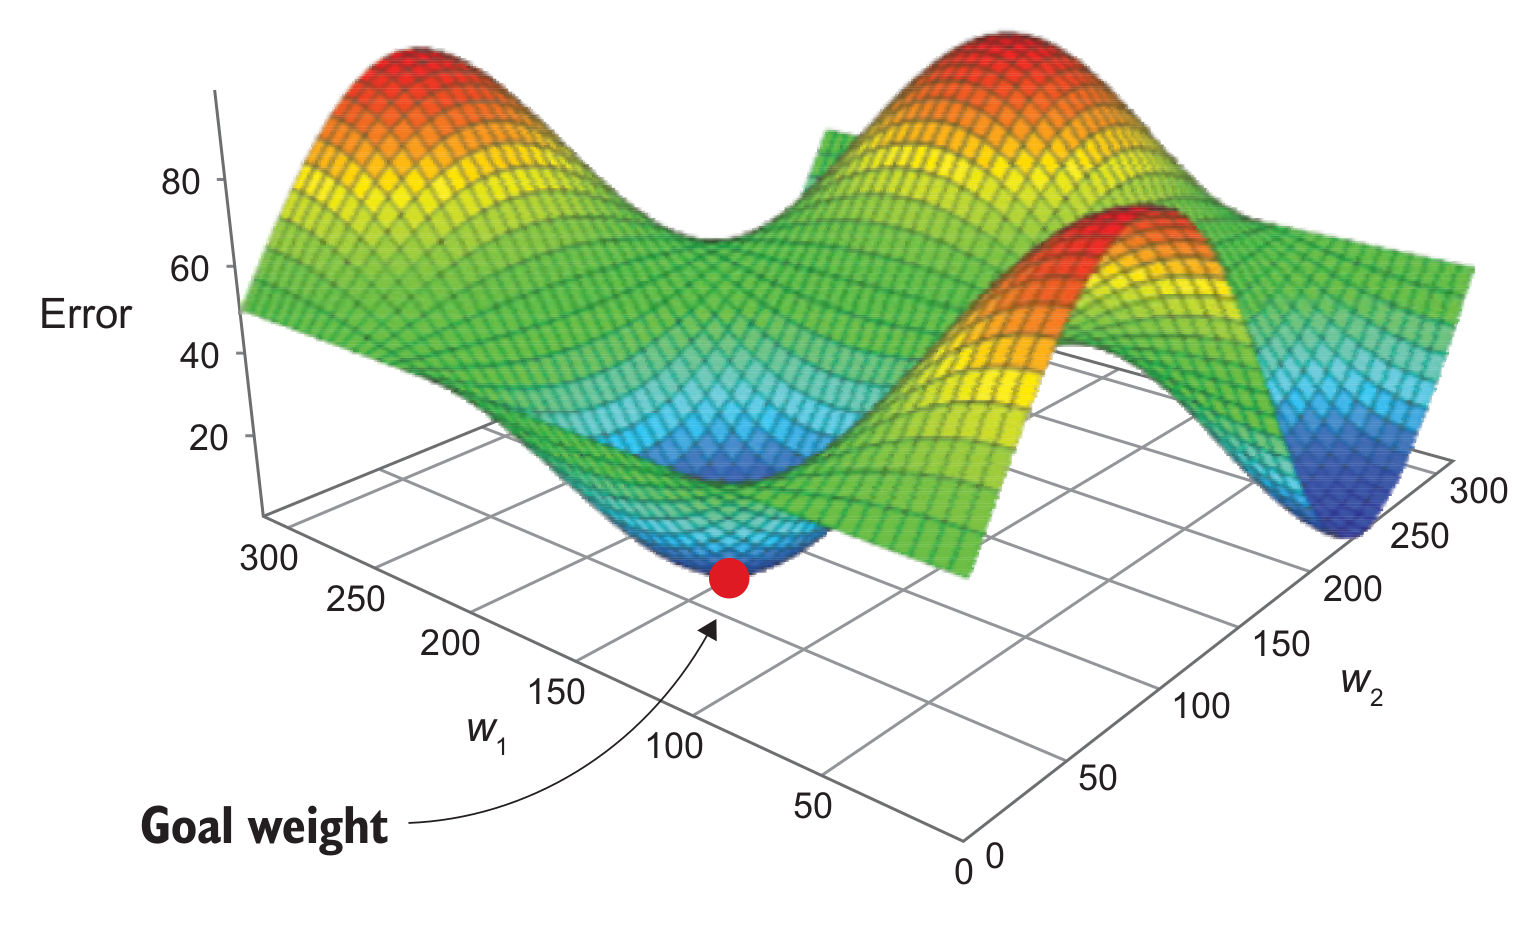
\includegraphics[scale=0.2]{images/cost-function-3d}
		\caption{The error function with respect to its weight for a single perceptron is a 2D curve}
	\end{figure}									
\end{frame}

\begin{frame}{Algoritma Optimasi (3/3)}
	\begin{figure}[ht]
		\centering
		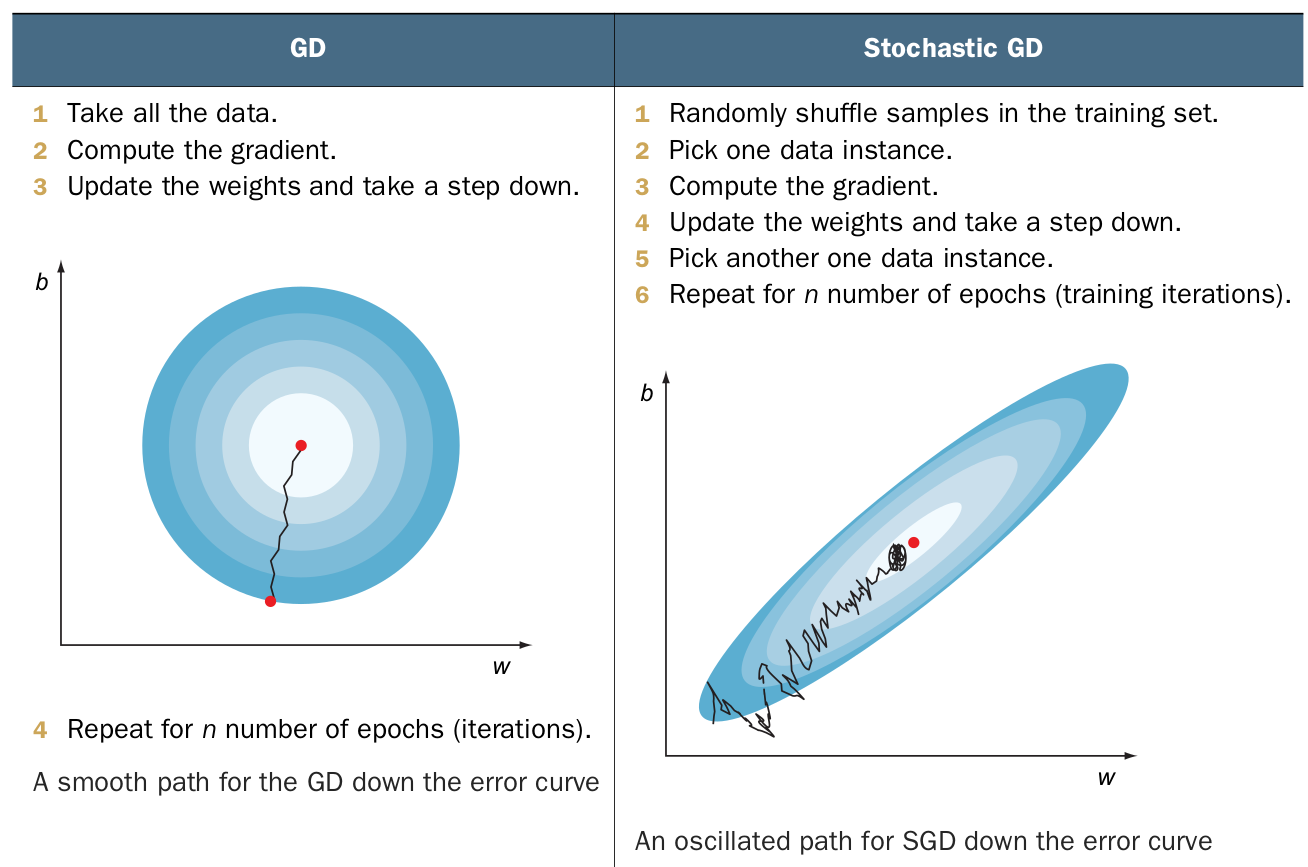
\includegraphics[scale=0.25]{images/gd-vs-stochastic}
	\end{figure}									
\end{frame}

\begin{frame}{Pitfalls of Batch Gradient Descent}
	\begin{figure}[ht]
	\centering
	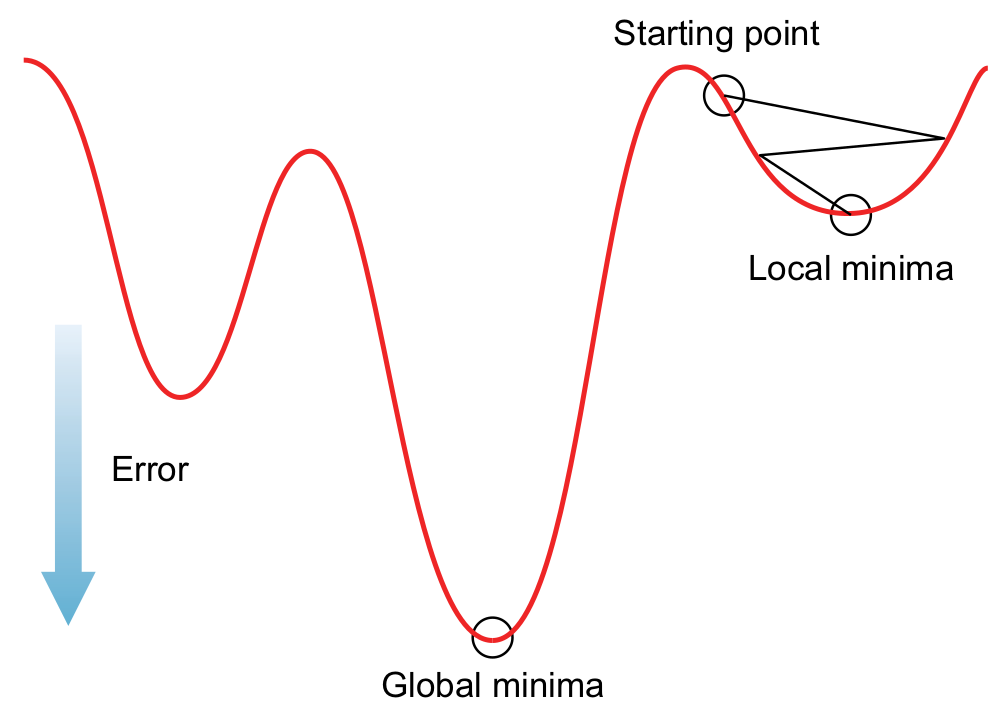
\includegraphics[scale=0.25]{images/pitfalls}
	\caption{Complex error functions are represented by more complex curves with many local minima values. Our goal is to reach the global minimum value.}
\end{figure}									
\end{frame}

\begin{frame}{Stochastic Gradient Descent}
	\begin{figure}[ht]
	\centering
	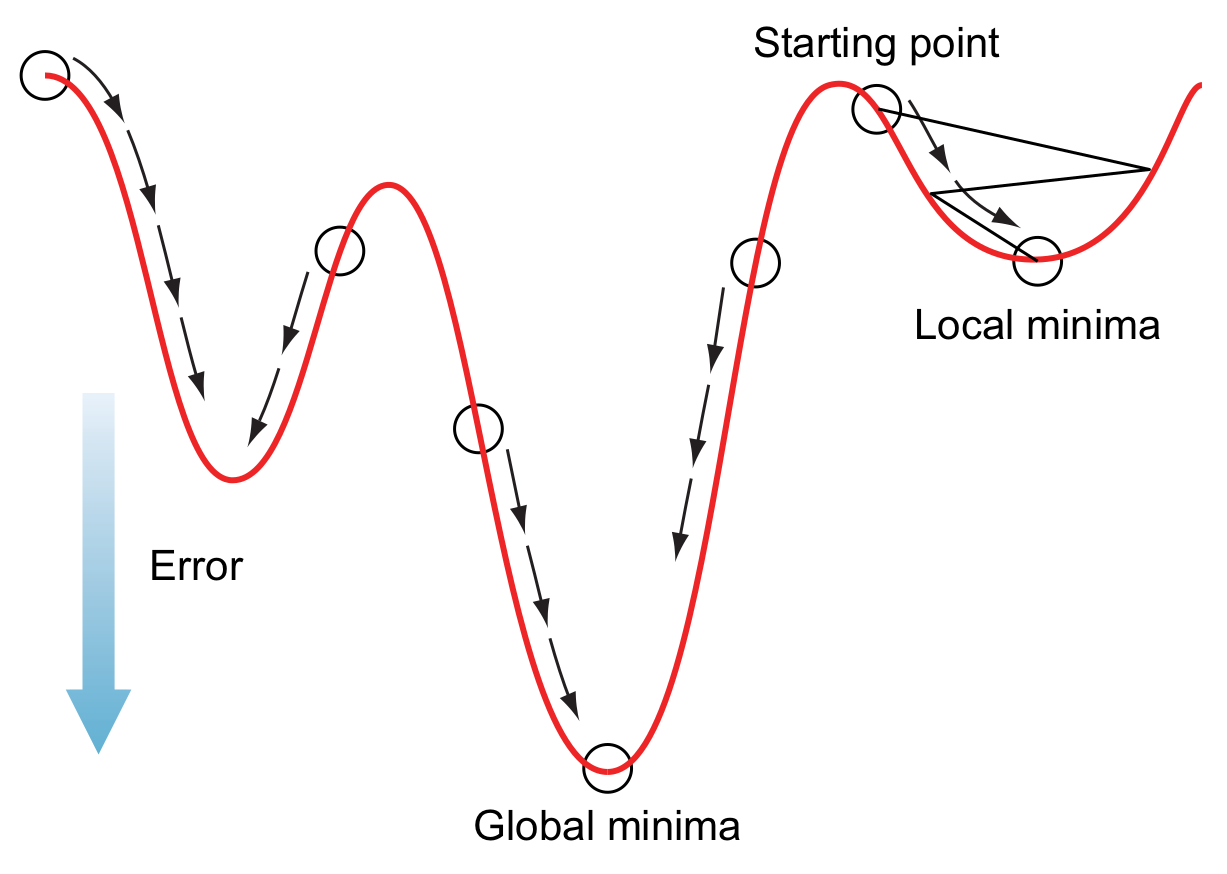
\includegraphics[scale=0.2]{images/stochastic-gd}
	\caption{The stochastic gradient descent algorithm randomly selects data points across the curve and descends all of them to find the local minima.}
\end{figure}	
\end{frame}

\begin{frame}{Mini-batch Gradient Descent}
	Mini-batch gradient descent (MB-GD) is a compromise between BGD and SGD.
\end{frame}

\begin{frame}{Gradient Descent Takeways (1/2)}
	\begin{itemize}
		\item<2-> Three types: batch, stochastic, and mini-batch.
		\item<3-> Batch GD updates the weights after computing the gradient of all the training data $\rightarrow$ computationally very expensive when the data is huge.
		\item<4-> Stochastic GD updates the weights after computing the gradient of a single instance of the training data $\rightarrow$ SGD is faster than BGD and usually reaches very close to the global minimum.
		\item<5-> Mini-batch GD is a compromise between batch and stochastic, using neither all the data nor a single instance. In most cases, MB-GD is a good starting point
	\end{itemize}
\end{frame}

\begin{frame}{Gradient Descent Takeways (2/2)}
	\begin{itemize}
		\item<2-> \texttt{batch\_size} is a hyperparameter that you will tune. You can start experimenting with \texttt{batch\_size = 32,64,128,256}.
		\item<3-> Don't get \texttt{batch\_size} confused with epochs. An epoch is the full cycle over all the training data. The batch is the number of training samples in the group for which we are computing the gradient. For example, if we have 1,000 samples in our training data and set \texttt{batch\_size = 256}, then epoch 1 = batch 1 of 256 samples plus batch 2 (256 samples) plus batch 3 (256 samples) plus batch 4 (232 samples).
	\end{itemize}
\end{frame}

\section{Backpropagation}
\begin{frame}{Backpropagation (1/3)}
	Training a neural network happens by the repetition of steps:
	\begin{itemize}
		\item<2-> Feedforward
		\begin{equation*}
			\hat{y} = \sigma \cdot W^{(3)} \cdot \sigma \cdot W^{(2)} \cdot \sigma \cdot W^{(1)} \cdot (x)
		\end{equation*} 
	\item<3-> Compare the prediction with the label to calculate the error or loss function:
		\begin{equation*}
			E(W,b) = \frac{1}{N} \sum_{i=1}^N{\left| \hat{y}_i - y_i \right|}.
		\end{equation*}			
	\item<4-> Use a gradient descent optimization algorithm to compute the $\Delta w$ that optimizes the error function:
		\begin{equation*}
			\Delta w_i = - \alpha \frac{dE}{dw_i}
		\end{equation*}
	\end{itemize}
\end{frame}

\begin{frame}{Backpropagation (2/3)}
		Backpropagate the $\Delta w$ through the network to update the weights:
		\begin{equation*}
			w_{\text{new}} = w_{\text{old}} - \alpha \left( \frac{dE}{dw_i} \right)
		\end{equation*}
\end{frame}

\begin{frame}{Backpropagation (3/3)}
	\begin{figure}[ht]
	\centering
	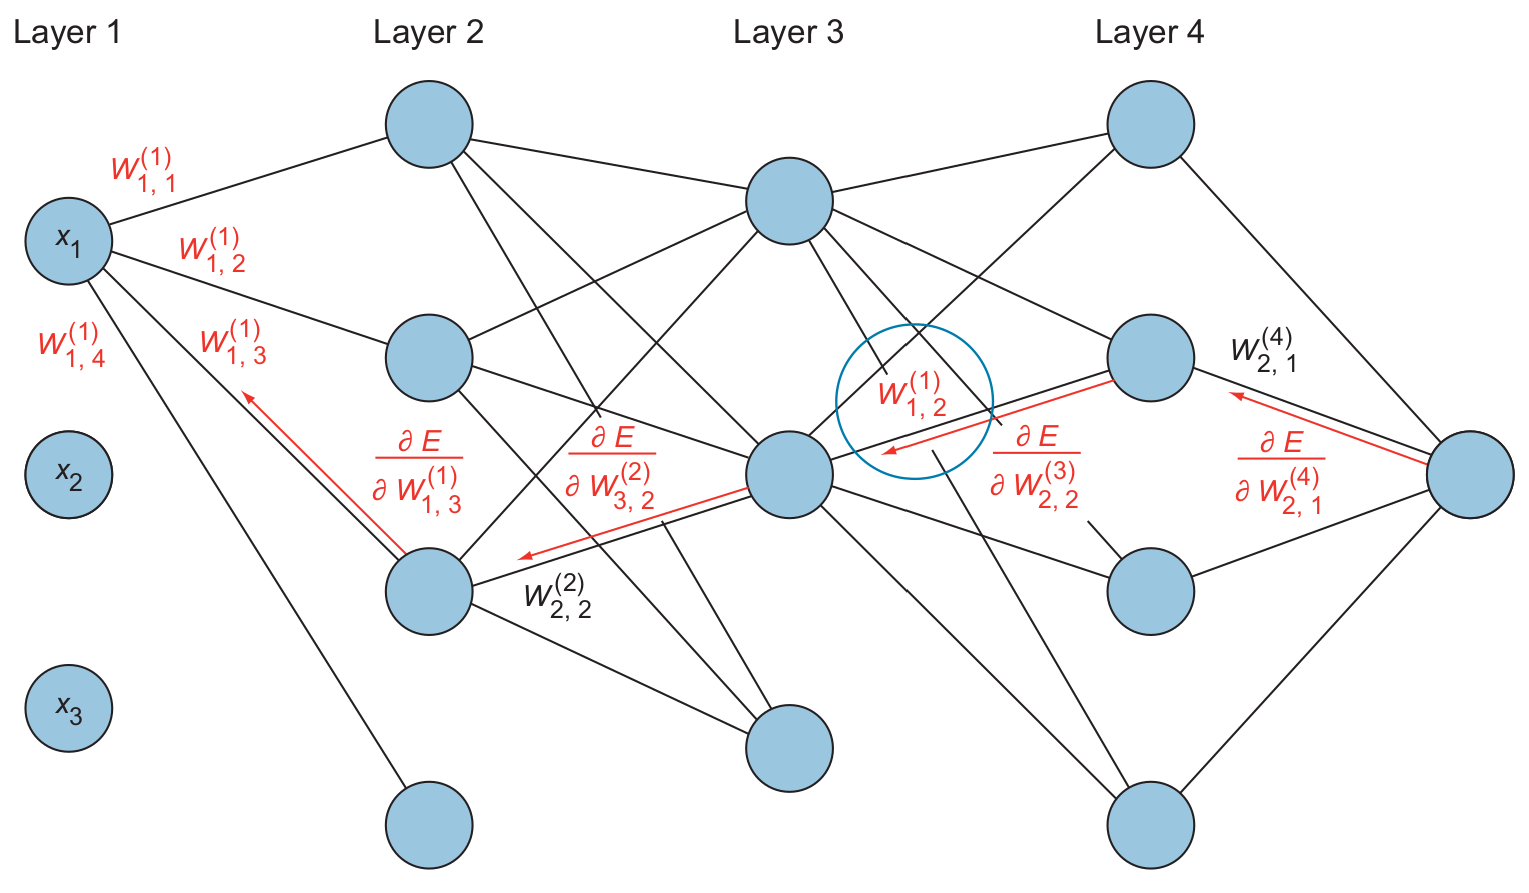
\includegraphics[scale=0.2]{images/chain-rule}
	\caption{Backpropagation uses the chain rule to flow gradients back through the network}
\end{figure}	
\end{frame}

\begin{frame}{Backpropagation Takeaways (1/3)}
	\begin{itemize}
		\item<2-> Backpropagation is a learning procedure for neurons.
		\item<3-> Backpropagation repeatedly adjusts weights of the connections (weights) in the network to minimize the cost function (the difference between the actual output vector and the desired output vector). 
		\item<4-> As a result of the weight adjustments, hidden layers come to represent important features other than the features represented in the input layer.
		\item<5-> For each layer, the goal is to find a set of weights that ensures that for each input vector, the output vector produced is the same as (or close to) the desired output vector. The difference in values between the produced and desired outputs is called the error function.
	\end{itemize}
\end{frame}

\begin{frame}{Backpropagation Takeaways (2/3)}
	\begin{itemize}
		\item<2-> The backward pass (backpropagation) starts at the end of the network, backpropagates or feeds the errors back, recursively applies the chain rule to compute gradients all the way to the inputs of the network, and then updates the weights.
	\end{itemize}
	\vspace*{-.5cm}
	\begin{figure}[ht]
	\centering
	\includegraphics<3->[scale=0.2]{images/forward-backward}
	\onslide<3-> \caption{The forward pass calculates the output prediction (left). The backward pass passes the derivative of the error backward to update its weights (right)}
\end{figure}	
\end{frame}

\begin{frame}{Backpropagation Takeaways (3/3)}
	\begin{itemize}
		\item<2-> To reiterate, the goal of a typical neural network problem is to discover a model that best fits our data Ultimately, we want to minimize the cost or loss function by choosing the best set of weight parameters.
	\end{itemize}
\end{frame}

\section{Lesson Summary}
\begin{frame}{Summary}
	\begin{itemize}
		\item<2-> Perceptrons work fine for datasets that can be separated by one straight line (linear operation). 
		\item<3-> Nonlinear datasets that cannot be modeled by a straight line need a more complex neural network that contains many neurons. Stacking neurons in layers creates a multilayer perceptron.
		\item<4-> The network learns by the repetition of three main steps: feedforward, calculate error, and optimize weights.
		\item<5-> Parameters are variables that are updated by the network during the training process, like weights and biases. These are tuned automatically by the model during training.
		\item<6-> Hyperparameters are variables that you tune, such as number of layers, activation functions, loss functions, optimizers, early stopping, and learning rate. We tune these before training the model.
	\end{itemize}
\end{frame}



%----------------------------%



%----------------------------%
% Conclusions
\begin{frame}
    \frametitle{}
    \centering
    
    \Large\color{oxfordblue}
    Thank you!

    \vspace{0.5cm}
    hendra.bunyamin@it.maranatha.edu

\end{frame}
%----------------------------%

% References slide
\begin{frame}
\frametitle{References}
\small
\bibliographystyle{apalike} %use the apalike bibliography style
\bibliography{references} % bibliography file
\end{frame}

%%%%%%%%%%%%%%%%%%%%
\end{document}
%%%%%%%%%%%%%%%%%%%%
